%!TEX root = Constructive Alignment for Introductory Programming.tex

\chapter{Approaches to Constructive Alignment} % (fold)
\label{cha:background}

\graphicspath{{Figures/Background/}}

This chapter reviews the existing literature related to constructive alignment, its theoretical foundations, applications in higher education, and relationship to published work in computing education research. The chapter aims to provide a general background on existing approaches to constructive alignment. Additional background literature is discussed in the following chapters in relation to the specific work presented. 

\sref{sec:constructive_alignment} provides background on constructive alignment, and relevant associated work on constructivism and aligned curriculum. This is followed in \sref{sec:reported_applications_of_constructive_alignment} with a systematic literature review of applications of constructive alignment reported in peer reviewed research publications, which outlines how others have approached the application of constructive alignment and their findings. \sref{sec:constructive_alignment_in_introductory_programming} then follows with a discussion of the challenges of teaching introductory programming, associated work from the computing education literature, and specifically looks at how constructive alignment has been applied for introductory programming. The chapter closes with \sref{sec:closing_comments} by briefly commenting on the opportunities for research that are addressed in the remainder of this thesis.


\section{Constructive Alignment} % (fold)
\label{sec:constructive_alignment}

Constructive alignment, as proposed by \citet{Biggs:1996c}, is an amalgamation of constructive learning theory and aligned instruction design. It aims to elicit deep learning approaches from all students. Biggs' model is student focused, with clear and intentional alignment of assessment, teaching and learning activities, and unit objectives. The central role of the learner in building meaning is derived from constructivist learning theories, whilst the alignment of assessment, teaching, and learning activities, has its foundation in instructional design literature. 

This section briefly describes these underlying principles and related literature, each of which is later expanded upon in \cref{cha:guiding_principles}. \sref{sub:approaches_to_learning} describes the work on approaches to learning, and discusses how the learning environment can influence students' approaches to learning. The central focus on constructive learning theories is then discussed in \sref{sub:constructivism}, with a discussion of aligned curriculum following in \sref{sub:aligned_curriculum}. The section concludes with an overview of the model of constructive alignment, \sref{sub:the_model_of_constructive_alignment}, and then a brief discussion of the example implementation of these principles that was presented by \citet{Biggs:1996c}.

\subsection{Approaches to Learning} % (fold)
\label{sub:approaches_to_learning}

The studies by \citet{Marton:1976a, Marton:1976b,Marton:2005} on student approaches to learning examined the processes and strategies students applied to learning. The work identified two different levels of processing, described as \emph{surface} and \emph{deep} approaches to learning, summarised in \tref{tbl:learning_approach}. When a student adopts a deep approach to learning, they study with the aim of understanding the material. They engage meaningfully with the task at hand, and use high cognitive levels in order to integrate the new knowledge into their current understanding. In contrast, when students use surface approaches to learning they engage lower cognitive levels, and aim only to be able to reproduce the material in test or exam conditions. When reading, for example, surface approaches can be characterised as focusing on the text itself, while deep approaches look for the meaning behind the text. Later work also added a third approach to learning termed a \emph{strategic} approach by \citet{Ramsden:1983}, or \emph{achieving} by  \citet{Biggs:1987}, identified students who switch between deep and surface learning approaches in order to maximise their grade. 

\begin{table}[h]
	\centering
	\caption{Approaches to Learning identified by \citet{Marton:1976a, Marton:1976b,Marton:2005}}
	\label{tbl:learning_approach}
	\begin{tabular}{l|l}
		\multicolumn{1}{c|}{\textbf{Deep}} & \multicolumn{1}{c}{\textbf{Surface}} \\
		\hline
		- Engage meaningfully & - Engage without meaning \\
		- High cognitive level & - Low cognitive level \\
		- Aim to integrate knowledge into self & - Aim to reproduce for assessment \\
		- Long term understanding & - Short term memorisation \\
	\end{tabular}
\end{table}

Marton and S\"{a}lj\"{o}'s work examined the different strategies students had used when adopting surface and deep approaches to learning, and attempted to provide activities designed to engage surface learners in similar activities to those adopting deep approaches \cite{Marton:2005}. For example, one strategy had the student answer questions similar to those spontaneously asked by students who had engaged in deep approaches to learning.  This strategy resulted in students adapting their surface learning approaches rather than in any change in the way they approached their studies. Students continued to ``skim the surface'' of the text, but in such a way as to be able to simply mention content from various sections in a very superficial way. 

An alternative strategy resulted in more positive results, as reported by \cite{Marton:1976b}. In this experiment, students were asked to read three chapters from a text with the aim of answering questions after reading that required either a) precise factual information, or b) broader understanding in terms of major lines of reasoning. Students who expected to answer factual questions tended to adopt surface approaches to learning. The group who expected broader questions had a mix of different approaches, with some adopting deep approaches, but not all. The major influencing factor had been the students interpretation of what was expected of them, with only half of the group interpreting the expectations as intended. 


A range of subsequent studies have associated deep approaches to learning with higher quality learning outcomes \cite{Rossum:1984,Prosser:1989,Trigwell:1991,Ramsden:1992,Marton:2005,DeRaadt:2005}. The work reported by \citet{DeRaadt:2005} related to the teaching of introductory programming, and used \citet{Biggs:2001} two-factor study process questionnaire (R-SPQ-2F) to evaluate the affect of study approach on results for one hundred and seventy seven students across eleven tertiary education institutions across Australia and New Zealand. The work found that \emph{approach to learning} had the strongest correlation to success as compared to other cognitive and demographic measures.

A student's perception of their learning environment has been found to influence the approach they take in their study. A range of investigations into students' perceptions of their learning environment, and its impact on the approach to learning, were reported by \citet{Ramsden:1992}. Shallow approaches were adopted by students who perceived assessment as requiring memorisation and recall, and by those who perceived workload to be high. Perceptions of high quality teaching, freedom in choosing some aspects of what is to be learned, and clarity of goals and standards required were all related to deep approaches \cite{Trigwell:1991,Ramsden:1992,Trigwell:1999}. These findings provide additional support for the original work of \cite{Marton:1976b}, that found that students adapt their learning approach based on what they perceive is expected of them.

\citet{Trigwell:1999} suggested that, given the observed relations between perceived environment and approach to learning, improvements in learning outcomes may be achieved by creating an environment that encourages and supports deep approaches.  Their work reported a number of important factors in creating this environment, including; teaching staff providing useful feedback, making objectives clear, motivating students and providing flexibility for students to determine what and how they learn. 

In their study of students' experiences learning to program, \citet{Bruce:2003} categorised the way students engage with learning to program into five categories, listed below. Each of these categories can be broadly classified as either a surface or deep approach to learning to program. When engaging surface approaches, students attempted to address the outcomes with as little effort as possible. This leads to situations in which students are primarily \emph{motivated} by fear of failing, and experience the learning as a struggle, with the topic appearing tedious, hard and boring, adjectives that are too often associated with learning to program \cite{McGettrick:2005}. On the other hand, when engaging deep approaches to learning students seek meaning in what they do, and relate their learning to the ``bigger picture.'' 

\begin{description}[noitemsep,nolistsep]
	\item[Surface Approaches] where student attention is on the parts and not the whole:
	\begin{description}[noitemsep,nolistsep]
		\item[Following] - ``getting through'' the unit becomes the students primary goal, and their focus is on completing assessment tasks without aiming to develop any level of understanding.
		\item[Coding] - rote memorisation of programming language syntax.
	\end{description}
	\item[Deep Approaches] attention is on programming as a whole:
	\begin{description}[noitemsep,nolistsep]
		\item[Understanding and integrating concepts] - students focus is on understanding programming concepts, and integrating these ideas to help with the development of programs.
		\item[Problem solving] -  programming is seen by the students as a means of solving problems, and their focus is on learning different ways to structure code to create solutions.
		\item[Participation/enculturation] - students aim to become programmers and to engage with the software development community and its culture.
	\end{description}
\end{description}

To succeed at learning to program, students need to engage deep approaches to learning, as surface approaches alone are unlikely to be sufficient \cite{Bruce:2003}. Pedagogy that allows us to encourage students to adopt deep approaches to learning should, therefore, help address some of the issues related to this challenging topic.

% subsection approaches_to_learning (end)


\subsection{Constructivism} % (fold)
\label{sub:constructivism}

Constructivism is a theory to explain the development of knowledge that focuses on the active role of the learner in constructing their own understanding. Dating back to \citet{Piaget:1950} constructivism exists in several forms: cognitive, individual, post-modern, radical and social constructivism \cite{Phillips:1995,Steffe:1995}. Each of these forms of constructivism has various implications for teaching and learning. Two review papers that discuss these implication are \citet{Jonassen:1991} and \citet{Vrasidas:2000}. These reviews outline the differences between constructivist and objectivist thinking in terms of education.

Approach to education is greatly influenced by the educator's theory of teaching and learning, with constructivist and objectivist theories often being seen at two extreme ends of a continuum. Objectivism is characterised by the presence of external meaning, or knowledge, and education is therefore a task for the learner to come to know that which is real \cite{Jonassen:1991,Vrasidas:2000}. Effective education can be realised through standardisation, and productivity improved through the mechanisms of management, as in business and industry \cite{Tyler:1969,Vrasidas:2000}. In contrast, constructivism is characterised by knowledge being internal to the learner, a human construction that is an interpretation of the external world \cite{Jonassen:1991,Vrasidas:2000}. Constructive teaching theories relate to guiding learners, helping them to adopt viable models with the aim of enabling them to think and act like experts. This suggests that effective education can be realised by creating an environment that gives students control over their learning \cite{Vrasidas:2000}. 

\begin{figure}[htpb]
	\centering 
	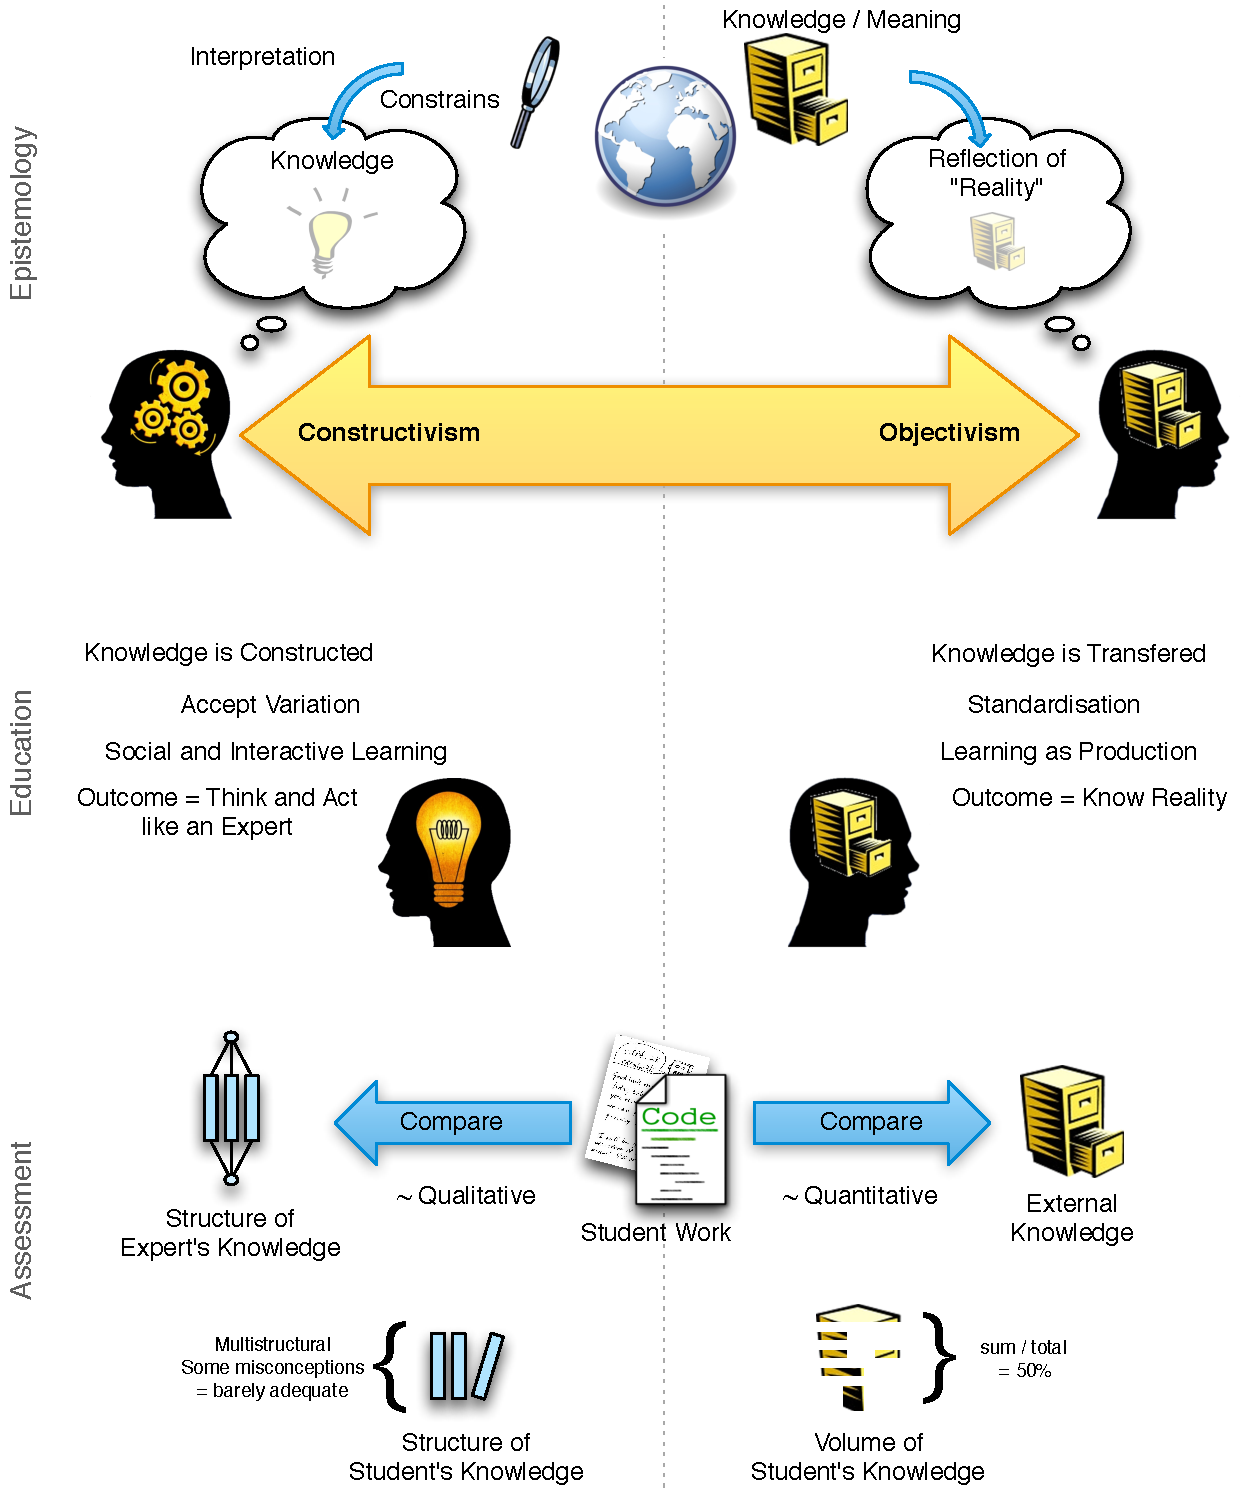
\includegraphics[width=\textwidth]{ConstructivismObjectivism}
	\caption{Illustration of the continuum from constructivism to objectivism, and the concepts present at levels of epistemology, education, and assessment.}
	\label{fig:const_obj}
\end{figure} 

The differences between constructivist and objectivist thinking are illustrated in \fref{fig:const_obj}. The illustration presents the characteristics of the two ends of the continuum, from constructivism on the left to objectivism on the right, related to epistemology, education, and assessment. 

\begin{description}[noitemsep,nolistsep]
	\item[Epistemology]: This section illustrates differences in how the two philosophical paradigms view knowledge
	\begin{itemize}[noitemsep,nolistsep]
		\item Constructivism is shown with knowledge being a human construction that is informed by observation of, and constrained by, external reality.
		\item Objectivism is depicted with human knowledge being a reflection of the external reality, the true source of knowledge.
	\end{itemize}
	\item[Education]: Shows differences between the two philosophical paradigms in terms of what makes effective education
	\begin{itemize}[noitemsep,nolistsep]
		\item Constructivism centres around guiding the learner's active construction of knowledge, with the objective of helping the learning think and act like an expert.
		\item Objectivism aims to effectively transfer knowledge to the learner, with the goal of them knowing reality.
	\end{itemize}
	\item[Assessment]: The final section of the illustration shows the different views on how to assess student understanding.
	\begin{itemize}[noitemsep,nolistsep]
		\item When guided by constructivism, assessment involves qualitatively evaluating the structure of the student's knowledge in relation to the structure of an expert's knowledge.  
		\item Adopting objectivism, assessment involves quantitatively evaluating the amount of external knowledge the student has managed to correctly retain.
	\end{itemize}
\end{description}

When education is guided by objectivism, instruction becomes the task of efficiently transferring knowledge to the learner. Material and tests can be standardised, using processes from business and industry to gain ``productivity-like'' improvements and to ensure the largest number of students are provided with access to the knowledge \cite{Tyler:1969,Vrasidas:2000}. Learning is seen as a matter of getting students to correctly conceptualise and categorise things, including the relationships between them \cite{Lakoff:1987}. It follows, therefore, that assessment is a matter of measuring the students behaviour against expectations. A focus on factual details is central to this extreme of the continuum. 

With constructivism, education is seen as creating a learning environment in which students will be exposed to situations that will enable their individual construction of knowledge \cite{Jonassen:1991,Vrasidas:2000}. Given that the student is constructing their own knowledge, context is important and prior experience shapes what a student learns \cite{Jonassen:1991a}. The goal is therefore to guide students in the construction of their knowledge, and to try to help them construct viable and meaningful conceptual structures \cite{Jonassen:1991,Vrasidas:2000}. Assessment, in constructivist thinking, is divergent as each student will bring their own ``reality'' and learning objectives therefore become less important and possibly irrelevant \cite{Jonassen:1992}. 

In relation to studies on effective teaching, constructivist learning theories -- with their student-centred focus -- appear to map well to features of productive learning environments. \citet{Martin:2000} reported a study of twenty six university teaching staff, considering how they intended to present a topic to their students and how they subsequently delivered the topic. Their results indicated that where staff conceived of the topic as ``knowledge as given'', they adopted teacher-focused information transmission forms of delivery consistent with objectivist theories. Given the findings discussed in \sref{sub:approaches_to_learning}, these strategies may result in students perceiving memorisation and recall as being what is required, and therefore adopt surface approaches to learning. Where the university staff viewed the object of study as related to conceptual change, a student-focused approach was taken, which is more consistent with constructivist thinking. When such approaches were adopted, learning tended to focus on higher cognitive level activities, with a broader focus on the discipline, practice or life-long-learning and encourage students to engage in deep approaches to learning.

% in programming

Early work on applying constructive learning theories to teaching computer science \cite{BenAri:1998,BenAri:2001} reported additional challenges in the application of constructivism due to the nature of computing. Beginner students in computer science have no \emph{effective model} of a computer to start with, instead beginning their study with a limited model akin to a ``giant brain.'' These inadequate models, and possible associated misconceptions, are likely to be exposed through interactions with the computer and possible ``psychological grief'' resulting as students work toward viable model. To address these issues, \citet{BenAri:1998,BenAri:2001} suggested the explicit teaching of a model of the computer, as originally proposed by \citet{DuBoulay:1986}. 

\citet{VanGorp:2001} provided a range of constructivist techniques suitable for teaching introductory programming, with the view of the constructivist classroom as a problem-solving environment. The work recommended students be provided authentic, though simplified, problems to help intrinsically motivate students, and that meaningful activities be designed to enable students in the construction of their own knowledge. Suggested activities included:

\begin{itemize}[noitemsep,nolistsep]
	\item \emph{Code walkthroughs} where students walk through existing code to predict computer behaviour.
	\item \emph{Code writing} where students produce small programs, small programs or pseudocode may be provided as \emph{scaffolding} for more complex tasks. 
	\item Location and correction of issues, both logical and syntactic, in the form of \emph{code debugging} activities.
	\item Greater interactivity was recommended for lectures, with students then being given time to \emph{reconstruct lecture notes} as a summarising activity. 
\end{itemize}


\citet{Thramboulidis:2003,Thramboulidis:2003a,Thramboulidis:2003b} described a shift from teaching a second programming unit on object oriented programming from a traditional ``textbook'' style approach, to a design-first approach based upon constructivist learning theories. The course presented by Thramboulidis involved students modelling familiar real-world situations using object oriented programming principles and class and sequence diagrams. This utilised students understanding of ``objects'' in the real world in the production of object oriented simulations suitable for implementation in computer programs. Following these activities, students went on to design and implement an object oriented calculator, making use of the concepts they had learnt from the earlier tasks. Results reported in this work indicated that the more active engagement of the students had resulted in positive improvements in both the pass rate and programs the students created. 

Constructivism has also been applied to teaching computer graphics, with mixed results. \citet{Taxen:2004} reported on a case study where they had applied constructive learning theories to teaching 3D graphics. The strategy applied in this work related to \emph{discovery learning} \cite{Duffy:1996} where teaching staff refrain from making explicit instruction, and instead provided a series of activities to help student discover the relevant knowledge themselves. The discussion and conclusions of \citet{Taxen:2004} indicated that students had felt the learning environment was too challenging, and they did not have sufficient background knowledge. Taxen's reflections indicated the use of an exam had contributed to a disconnect between the teaching approach and the assessment approach; the exam, in effect, encouraged students to adopt surface approaches that had been actively discouraged in the learning.

\citet{Wulf:2005} reported a constructivist-based pedagogy for teaching introductory programming and information technology that was considered to have created a more accessible environment for a wider range of students. This work recommended the active learning tasks outlined by \citet{VanGorp:2001}, and expanded upon this with a studio-based approach to teaching introductory programming with collaborative group-based instruction to create a more student-centred learning environment for computer science units.

These various works on constructivism in computer science education indicate that the application of constructivist learning theories should be beneficial for teaching introductory programming. By focusing on the active role of the student in constructing their own knowledge it should be possible to create a unit in which students develop an appropriate model of the computer, gain an understanding of important programming concepts, and acquire associated programming skills.

% subsection constructivism (end)

\subsection{Aligned Curriculum} % (fold)
\label{sub:aligned_curriculum}

\citet{Tyler:1969} defined curriculum alignment as occurring when material learnt in earlier years is built upon and supported in subsequent classes. Tyler's aligned model consisted of four major steps (1) identifying objectives, (2) choosing appropriate learning experiences, (3) organising these experiences so as to maximise learning, and (4) evaluating the resulting learning. These four steps were always aligned, with objectives matching experiences and assessment tasks. The work of \cite{Ramsden:1992} indicates that this alignment can be achieved as long as assessment matches objectives; from the students perspective the curriculum is always defined by the assessment.

Benefits of aligned curriculum can be related to the work on approaches to learning. One of the identified requirements for positive learning environments, discussed in \sref{sub:approaches_to_learning}, was the clear communication of expectation to students. In an aligned curriculum the teaching and learning activities match the assessment tasks, and help provide the clarity of intention required to encourage students to engage in deep approaches to learning.

The impact of aligning teaching and learning activities and assessment tasks was highlighted by \citet{Cohen:1987}. In discussing instructional alignment \citet{Cohen:1987} reported students achieved significantly better results when the teaching was aligned to the assessment than with non-aligned instruction. This is in line with expectations if an aligned curriculum is likely to help engage students appropriately with learning tasks.

% subsection aligned_curriculum (end)

\subsection{The Model of Constructive Alignment} % (fold)
\label{sub:the_model_of_constructive_alignment}

Constructive alignment brings together aspects of constructive learning theories together with aligned curriculum, with the overall aim of encouraging students to adopt deep approaches to learning.

In his original paper on constructive alignment \citet{Biggs:1996c} adopted constructivism as a framework to help guide decision making in all facets of teaching and learning. Constructivism was chosen due to its central focus on the students construction of their own knowledge, and the student-centred learning environments that result from accepting this epistemology. \citet{Biggs:1996c}, clarified again in \citet{Biggs:2007}, makes it clear that the emphasis is on student activity being central to knowledge construction, and that education should focus more on \emph{conceptual change} than on acquisition of information. This pragmatic view places Biggs' work somewhere on the constructivist side of the constructivism-objectivism continuum, but not necessarily at its extreme. 

\emph{Aligned curriculum} forms the second pillar of constructive alignment. \citet{Biggs:1996c} proposed the alignment of teaching and learning activities and assessment tasks to a unit's intended learning outcomes. Intended learning outcomes capture unit\footnote{A unit in this context refers to a unit of study, also called a subject or course in other institutions.} goals in terms of cognitive activities students will be able to perform by the end of the unit. Biggs' work claimed that this use of aligned curriculum -- with constructivist learning theories -- results in a student-centred learning environment and a clear focus and consistent message.

\citet{Houghton:2004} described an overall model of constructive alignment, illustrated in \fref{fig:Houghton}, as consisting of the following blocks:
\begin{itemize}[noitemsep,nolistsep]
	\item \emph{Intended learning outcomes} clearly define required learning in terms of ``performances of understanding.''
	\item \emph{Performance objectives} emerge from the desired outcomes, and can be ranked to become the assessment criteria.
	\item \emph{Teaching and learning activities} are designed to place students in situations likely to elicit the required learning.
	\item Students provide \emph{evidence of their learning}, that are assessed against the criteria to determine grade outcomes.
\end{itemize}

\begin{figure}[htpb]
	\centering 
	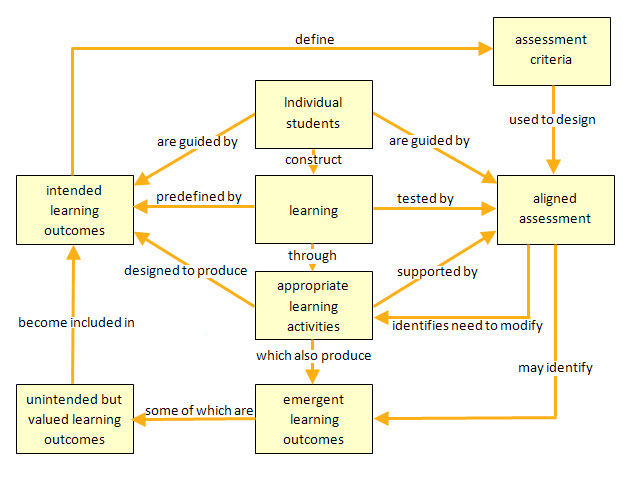
\includegraphics[width=\columnwidth]{Houghton_constructive_alignment_1}
	\caption{Constructive alignment model presented by \citet{Houghton:2004}}
	\label{fig:Houghton}
\end{figure}

Intended learning outcomes are central to constructive alignment, and therefore their construction must ensure suitable cognitive levels are required in order to encourage deep approaches to learning. \citet{Biggs:1996c} proposed the use of the SOLO taxonomy \cite{Biggs:1982} for this purpose. SOLO stands for \emph{Structure of the Observed Learning Outcome} and defines five levels of outcomes: pre-structural, uni-structural, multi-structural, relational and extended abstract. These levels are illustrated in \fref{fig:solo} and described in the following list. Each of the five levels of outcomes can be associated with a list of verbs likely to elicit that level of cognitive activity, and these verbs can then be used in defining a unit's intended learning outcomes.

\begin{description}[noitemsep,nolistsep]
 	\item[Prestructural] indicates no understanding of the topic; essentially, the student has \emph{missed the point}.
 	\item[Unistructural] indicates understanding of one relevant aspect of the topic; the student starts addressing the topic but does little more than \emph{get on track}.
 	\item[Multistructural] indicates understanding several relevant aspects, but each is understood in isolation. The student can provide a suitable list of facts, but does not structure their response to address the topic as a whole. To adopt clich\'{e}, the student ``sees the trees but not the forest.''
 	\item[Relational] understanding indicates that the topic is seen as a whole, with the various aspects integrated into a relevant structure. The student can respond appropriately to questions, demonstrating an integrated understanding of the topic.
 	\item[Extended Abstract] goes beyond the present, generalising the structure into new domains or in new ways. The student should be able to demonstrate a ``breakthrough'' response providing new insights on the topic.
\end{description} 

\begin{figure}[htbp]
	\centering
	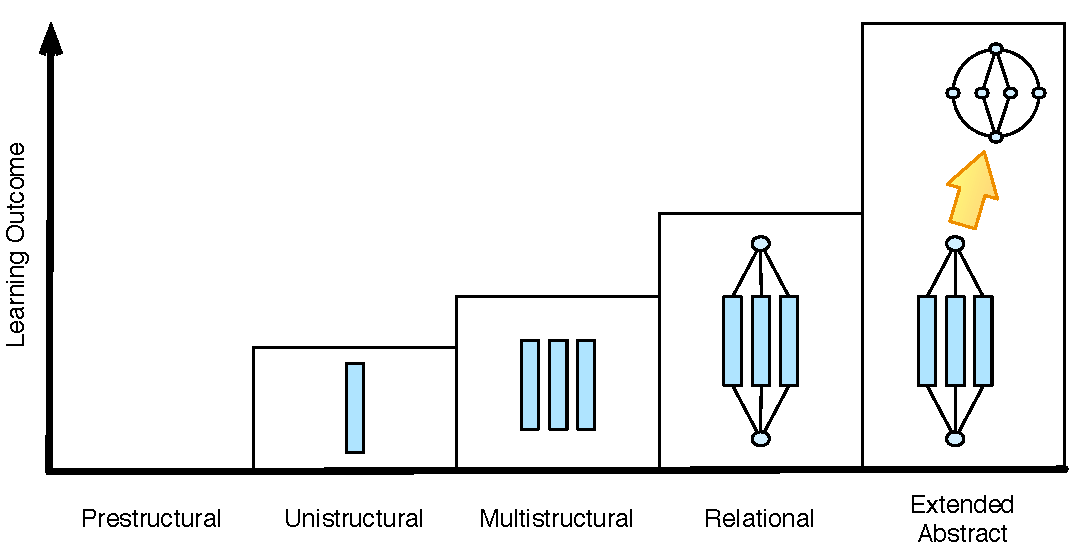
\includegraphics[width=0.9\textwidth]{SOLO}
	\caption{The five levels of the SOLO taxonomy, used to help define intended learning outcomes and assessment criteria, adapted from \citet{Biggs:2007}.}
	\label{fig:solo}
\end{figure}

Constructive alignment aims to encourage students to engage in deep approaches to learning by clearly stating unit intended learning outcomes, aligning teaching and learning activities and assessment tasks with these outcomes, in a student-centred environment. In this way, constructive alignment helps communicate to students the required approach to learning, with a consistent message throughout delivery and assessment. The resulting student-centred environment weaves a ``web of consistency,'' optimising the likelihood of students \emph{engaging appropriately} with learning activities \cite{Biggs:1999}.

% subsection the_model_of_constructive_alignment (end)

\subsection{Biggs' Example Implementation} % (fold)
\label{sub:biggs_example_implementation}

Interestingly, the principles of constructive alignment were not conceived and then implemented, but rather \emph{discovered} through reflection. \citet{Biggs:2007} (p.51) describes the discovery of these principles through the application of a portfolio for assessment of a third year psychology unit in the Bachelor of Education, the compelling example used in \citet{Biggs:1996c} and further elaborated upon in \citet{Biggs:1997}.

\citet{Biggs:1997} described a portfolio as a body of work selected by the student to demonstrate that they had met the unit's intended learning outcomes. A portfolio consisted of a number of \emph{items}, or \emph{pieces} of work, as well as an overall statement indicating \emph{why} the items had been included, and how they demonstrated that the student had met the unit's intended learning outcomes. Portfolios are discussed in further detail in \sref{sub:portfolio_assessment}.

Biggs' example of constructive alignment clearly demonstrated the application of both constructive learning theories, and aligned curriculum. By using a portfolio, the unit revolved around the intended learning outcomes, with students needing to submit a body of work that demonstrated how they had met outcomes in order to pass the unit. The portfolio was assessed holistically, with different grade outcomes relating to how well the learning outcomes had been addressed. Teaching and learning activities revolved around the preparation of portfolio pieces, including a range of student centred activities and guided instruction where appropriate.

\citet{Biggs:1996c} indicated that the results from the first implementation of the example application of constructive alignment had ``stunning'' results; portfolios included a range of rich and exciting evidence of learning, a large number of students received high grades, and student feedback was the best the unit had received. Biggs attributed this success to the design of the unit. Intended learning outcomes had defined required performance levels, teaching and learning activities had elicited them, and assessment had confirmed them. The assessment, activities, and outcomes had been in alignment, all working together to help the students construct the required knowledge. These aspects then formed the formal pillars of the constructive alignment model proposed by Biggs.

% subsection biggs_example_implementation (end)

% section constructive_alignment (end)

\clearpage
\section{Reported Applications of Constructive Alignment} % (fold)
\label{sec:reported_applications_of_constructive_alignment}

In this section we outline a literature review that examines some applications of constructive alignment in Higher Education. This review aims to identify how constructive alignment can be applied to introductory programming, and any gaps in the current research literature. 

\subsection{Review Method} % (fold)
\label{sub:review_method}

\citet{Petticrew:2008} defined a systematic literature review as a process of systematically analysing all available studies in order to answer specific research questions. The systematic nature of reviews carried out in this manner ensure that the review is thorough and fair, providing an opportunity to synthesise existing work in a scientific manner. The review presented here followed the systematic literature review process of \citet{Kitchenham:2004}, and aimed to identify, to the best of our knowledge, all available studies on how Constructive Alignment has been applied in Higher Education.

\fref{fig:struct_review_proc} shows the three phases in the systematic literature review carried out in this work. The first phase identified appropriate search and filter criteria used in locating associated literature. In Phase 2, the search criteria was used to identify potentially relevant articles from the indicated sources. The articles identified were then filtered, using the filter criteria, to identify the relevant articles to pass on to Phase 3, where relevant data was collected from the articles, and the results analysed.

\begin{figure}[tbph]
	\centering
	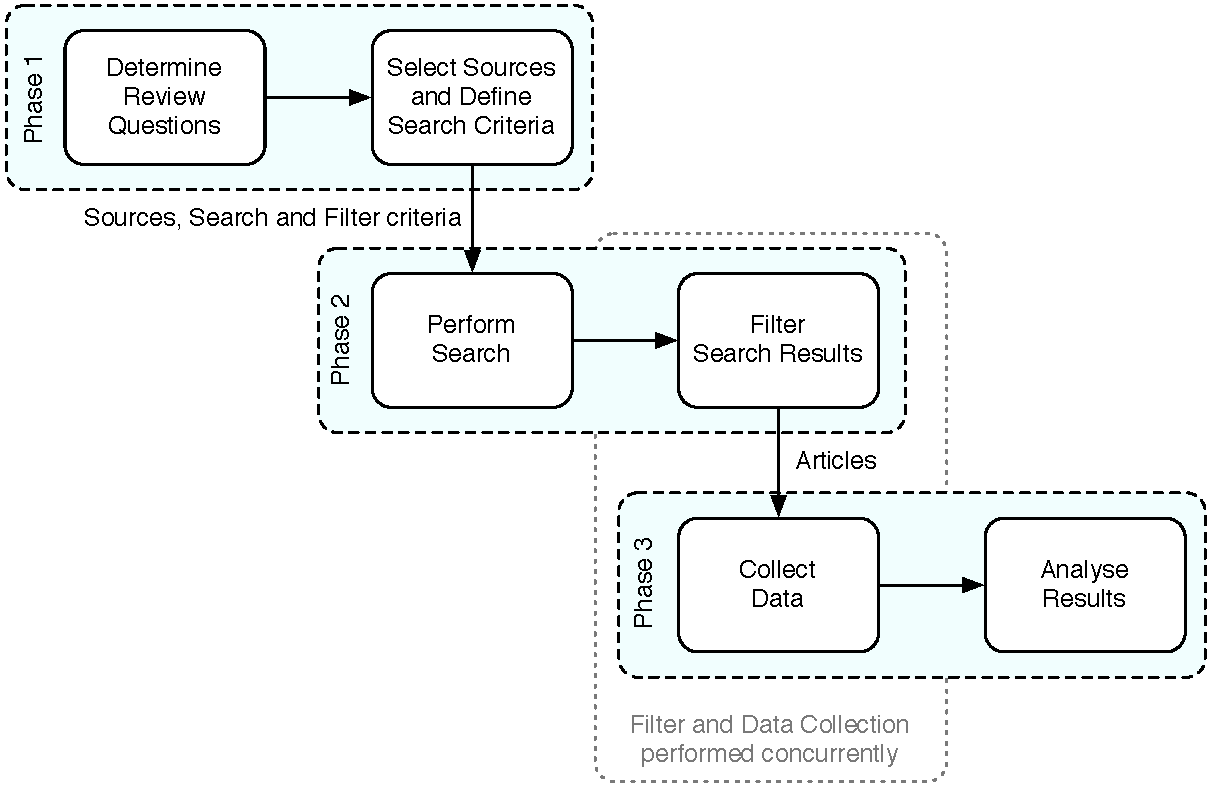
\includegraphics[width=\textwidth]{SystematicReview}
	\caption{Systematic Literature Review processes carried out in this work, based on steps of \citet{Kitchenham:2004}.}
	\label{fig:struct_review_proc}
\end{figure}



\subsubsection{Phase 1: Search and Filter Criteria} % (fold)
\label{sub:review_questions}

This review focused on the application of constructive alignment, and the effectiveness of the teaching and learning environment created. \citet{Petticrew:2008} suggested that the formulation of research questions for a systematic review should consider five aspects: Population, Intervention, Comparison, Outcome and Context (PICOC). Addressing these five aspects enabled the creation of effective search and filter criteria.

\tref{tbl:picoc} lists the five PICOC aspects related to this review. The Population consists of the specific target group that the study examines. In this study the population included students and academics in the context of Higher Education. This work aimed to review interventions where academics had applied the principles of constructive alignment, and any comparisons they had with existing approaches to teaching and learning. It aimed to investigate the range of approaches to delivery, and kinds of assessment used. In terms of outcomes, we were interested in examining any positive or negative impacts these changes had on either staff or students.

\begin{table}[t]
	\renewcommand{\arraystretch}{1.2}
	\centering
	\caption{Focus ``aspects'' for database search using PICOC}
	\label{tbl:picoc}

    \begin{tabular}{l|p{9cm}}
    \textbf{Aspect} & \textbf{Value} \\
    \hline
    Population & Students and Academics in Higher Education\\
    Intervention & Applications of Constructive Alignment in the design of teaching and learning activities and assessment. \\
    Comparison & Existing approaches \\
    Outcomes & Positive and negative impacts on student learning, as well as impacts on teaching staff. \\
    Context & Application of Constructive Alignment to the design and delivery of teaching and learning material in a Higher Education setting. \\
    \end{tabular}
\end{table}


This systematic literature review aimed to answer the following questions:

\begin{enumerate}[noitemsep,nolistsep]
	\item What evidence is there of studies on the application of constructive alignment to teaching and learning in higher education?
	\item How has the effectiveness of constructive alignment been measured in these studies, and how effective has constructive alignment been in the higher education setting?
	\item What teaching and learning activities were used in conjuncture with constructive alignment?
	\item What forms of assessment have been used with constructive alignment?
	\item In what ways have applications of constructive alignment addressed the two main elements of constructive alignment: constructivism and aligned curriculum?
\end{enumerate}

\citet{Petticrew:2008} described the need for the search criteria to result in high number of relevant articles, while excluding irrelevant ones. This is referred to as the search criteria \emph{sensitivity} and \emph{specificity}. A search with high sensitivity returns a high number of relevant articles, with high specificity a low proportion of irrelevant articles. While an ideal search criteria would be both highly sensitive and highly specific, in practice there generally tends to be a trade-off between the two. 

\citet{Kitchenham:2004} provides a number of recommendations on how to define appropriate search criteria, including the use of Boolean AND and OR conditions as well as searching for synonyms. Using this approach results in a search with higher specificity, and can result in a low number of articles being identified, see \citet{Salleh:2011} for example. Therefore, for this work it was decided to start with a highly \emph{sensitive} search criteria, and search for articles that match the term ``Constructive Alignment.'' If this resulted in a unacceptably large number of results then more specific criteria could have been added.

Given the highly sensitive search criteria, a high number of irrelevant articles was anticipated. To address this, Phase 1 also defined a number of filter conditions. The aim of these conditions was to clearly define why papers would be excluded from the analysis in Phase 3. The following lists the criteria used.

\begin{itemize}[noitemsep,nolistsep]
	\item The full text of the paper must be available to the researchers, and must be published in English.
	\item The paper must appear in a peer reviewed conference, journal or workshop.
	\item Constructive Alignment must be discussed either as the main focus, or an important aspect, of the paper.
	\item Results must relate to the use of Constructive Alignment in a teaching and learning context.
\end{itemize}

% subsection research_questions (end)

\subsubsection{Phase 2: Identification of Relevant Literature} % (fold)
\label{ssub:identification_of_relevant_literature}

In Phase 2, the search and filter criteria from Phase 1 were used to carry out the search on the selected online databases. The resulting articles were collected in an academic reference management system that allowed articles to be categorised using a status and a number of tags. Categories were created to indicate why a paper had been excluded, and to mark each paper's progress through the data collection. 

Database searches were performed within the reference management system, which provided facilities to automate the collection of the citation data and the associated full text. Where the full text was not available from the database, a general search was performed using a number of search engines in order to ensure the full text was included for as many articles as possible. This import process also identified any references that were already included in the system, thereby avoiding the creation of duplicates in the resulting library.

The use of the categorisation tools in the academic reference management system allowed the Filter stage of Phase 2 and the Data Collection stage of Phase 3 to run concurrently. Once imported, each article was placed in a \textbf{To Be Categorised} status, thereby providing a backlog of the articles that were to be examined. Each of these articles was then examined using the filter criteria, and moved to a separate status as the filter process progressed. The stages of this process are shown in \fref{fig:filter_proc}.

\begin{figure}[tbph]
	\centering
	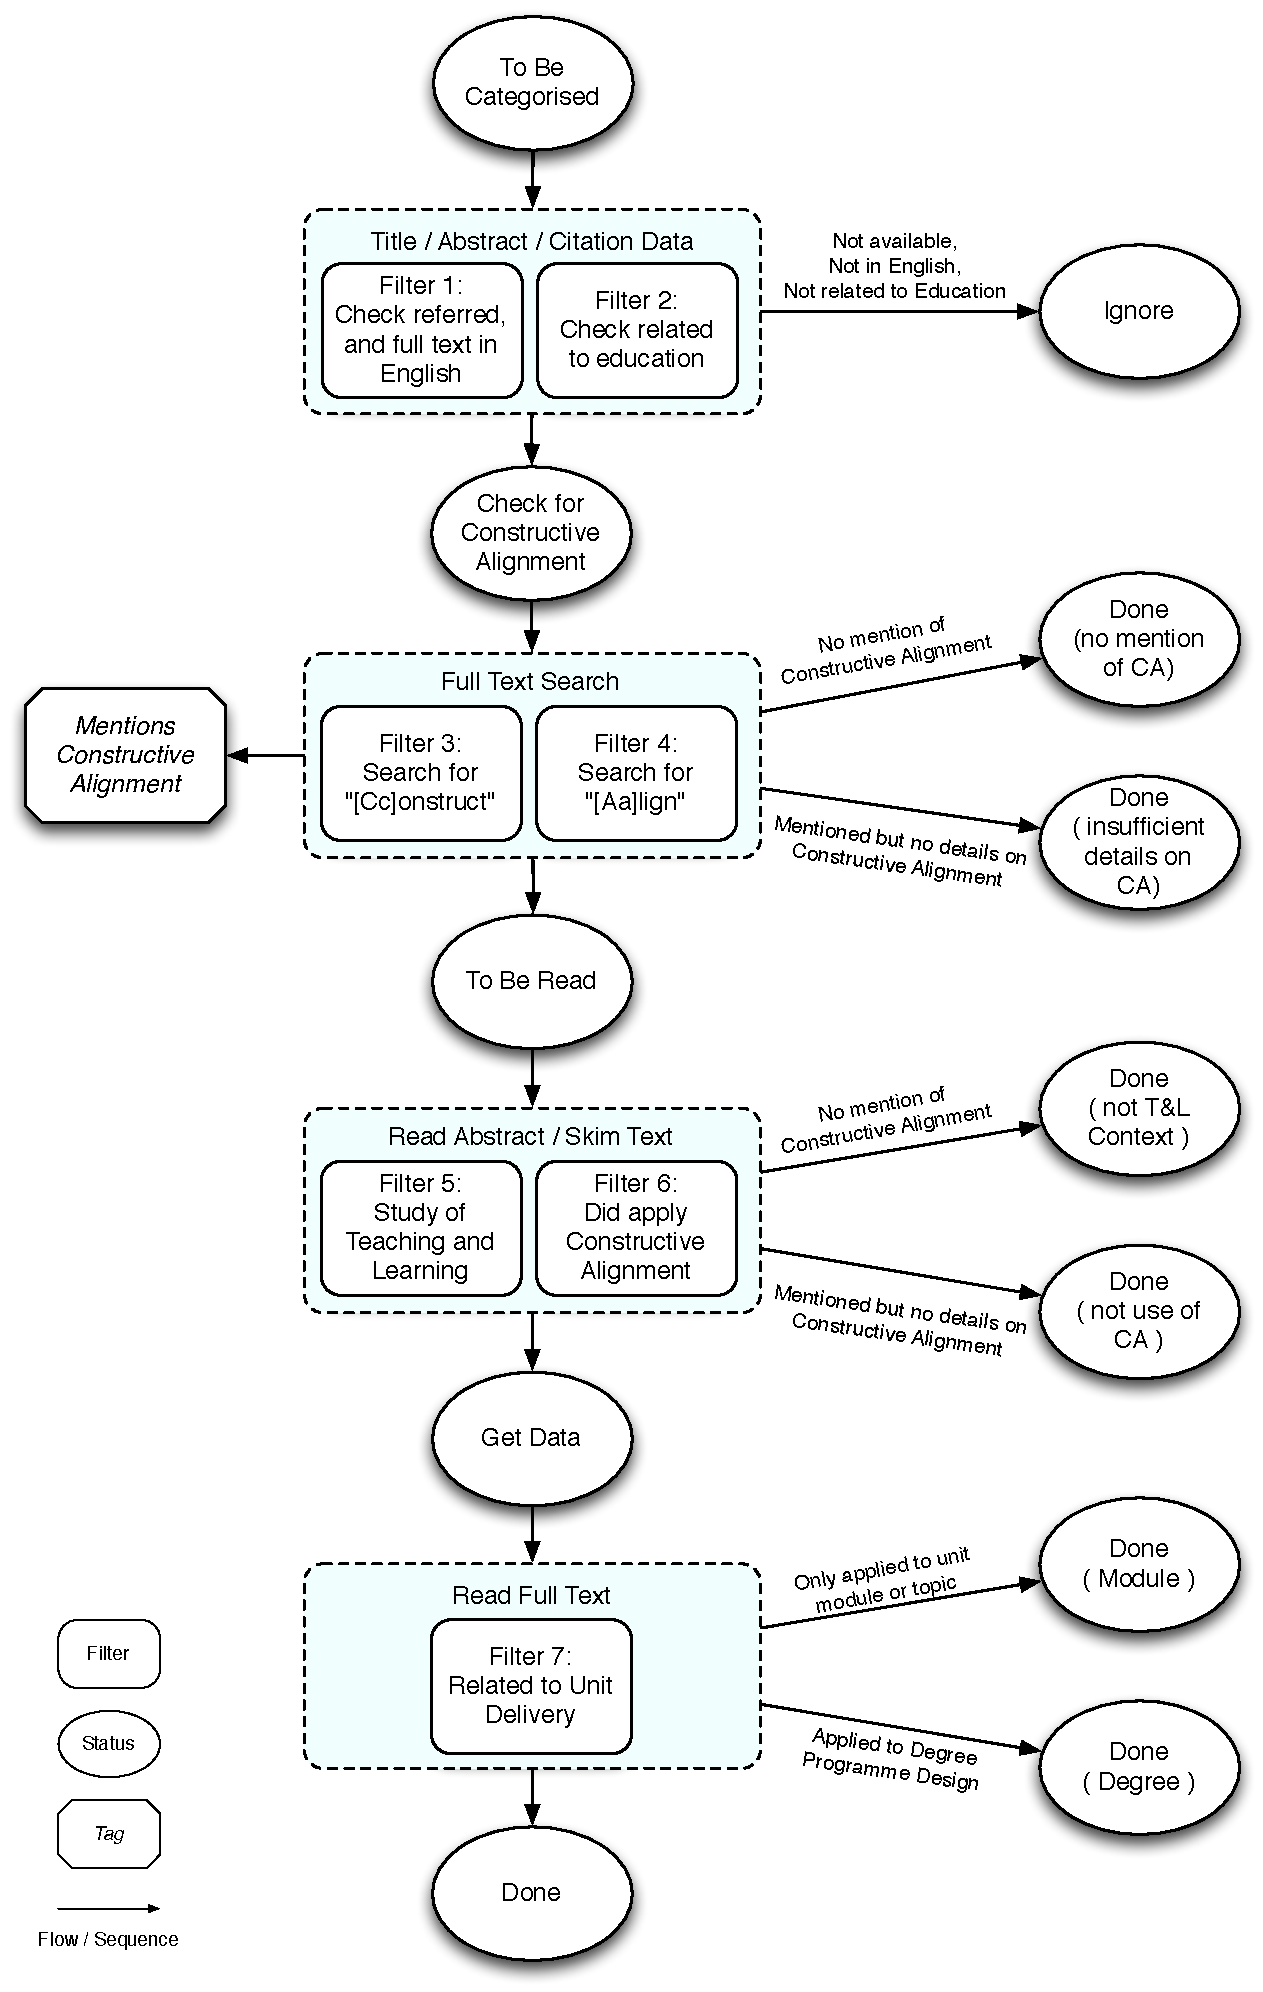
\includegraphics[width=0.8\textwidth]{FilterProcess}
	\caption{Filter process applied to papers}
	\label{fig:filter_proc}
\end{figure}

In the first stage of the filter process the availability of full text, the language it was written in, and its refereed status was checked. If these were not met the paper was allocated to the \textbf{Ignore} status, and did not proceed to the next stage of the filter. 

At the next stage a full text search was conducted on each paper. This search looked for the presence of any text related to constructivism or alignment through the search strings ``construct'' and ``align.'' The associated text was then read, and the paper was allocated to \textbf{Done (no mention of Constructive Alignment)} when there was no presence of either words, to \textbf{Done (insufficient details on Constructive Alignment)} when it was mentioned briefly with no details or in depth discussion, and to \textbf{To Be Read} in all other cases. % All papers that had mentioned Constructive Alignment were tagged at this stage.

Stage 3 involved reading the abstracts, and all sections related to Constructive Alignment from the papers in the To Be Read status. A new status was allocated to each paper: \textbf{Done (not a Teaching and Learning Context)} if they were a discussion of education theory rather than a study of a teaching and learning context, \textbf{Done (not an application of Constructive Alignment)} if they mentioned Constructive Alignment but had not adopted it for the reported work, and \textbf{Get Data} in all other cases.

The final stage involved reading the full text of the papers that had been marked with the Get Data status, and classifying them based on what Constructive Alignment had been applied to. Data was collected from all of the papers at this stage, but only those related to the delivery of a unit were forwarded to the analysis phase.

% subsubsection identification_of_relevant_literature (end)

\subsubsection{Phase 3: Data Collection and Analysis} % (fold)
\label{ssub:data_collection_and_analysis}

Data collection was performed by reading the indicated papers and looking for the details in the following list. Findings were recorded in a spreadsheet for further analysis, with relevant quotes from the text stored alongside the summarised information.

\begin{itemize}[noitemsep,nolistsep]
	\item Level of Unit: Undergraduate or Postgraduate, and year level.
	\item The Intended Learning Outcomes and associated levels from the SOLO taxonomy.
	\item Teaching and Learning activities used.
	\item Approach to assessment.
	\item Reported effects of constructive alignment.
\end{itemize}

In keeping with the holistic nature of the assessment approaches suggested in \cite{Biggs:1997}, the quality measure for each paper was generated by response to the following question using a five point Likert scale \cite{Likert:1932}: 5 being strongly agree, 4 agree, 3 neutral, 2 disagree, and 1 strongly disagree.

\begin{quote}
``The paper clearly communicates how constructive alignment was applied to the unit, and the results obtained. ''	
\end{quote}

Once all of the data had been collected the details were summarised in a spreadsheet, and analysed to answer the review questions.

% subsubsection data_collection_and_analysis (end)


% subsection review_method (end)
\clearpage
\subsection{Results} % (fold)
\label{sub:review_results}

The search involved the use of seventeen online databases, all of which were searched for the term ``Constructive Alignment.'' \tref{tbl:review_source} lists the number of results from each of the selected databases. Google Scholar (\url{http://scholar.google.com}) and CiteSeer (\url{http://citeseerx.ist.psu.edu}) resulted in an overly large number of articles for the selected search term. In both cases the results appears to have a large number of irrelevant matches, and so the search terms were made more specific. The search in Google Scholar was updated to search for articles that included ``Constructive Alignment'' in the title, while CiteSeer was limited to searching abstracts for the associated text.

\begin{savenotes}
\begin{table}[htb]
	\centering
	\caption{Data sources and the number of articles located for the search term ``Constructive Alignment''}
	\label{tbl:review_source}
	\footnotesize
    \begin{tabular}{l|l|c}
    \textbf{Source} & \textbf{URL} & \textbf{Count} \\ \hline
    A+ Education & \url{http://search.informit.com.au/search} & 44 \\
    Academic Search Complete & \scriptsize \url{http://ebscohost.com/academic/academic-search-complete} & 32 \\
    ACM Digital Library & \url{http://dl.acm.org} & 21 \\
    CiteSeer\footnote{Within CiteSeer the search was performed on article abstracts containing the text ``Constructive Alignment.''}  & \url{http://citeseerx.ist.psu.edu} & 20 \\
    EdResearch Online & \url{http://opac.acer.edu.au:8080/edresearch} & 6 \\
    \scriptsize Educational Research Abstracts & \url{http://www.tandfonline.com} & 26 \\
    \scriptsize Education Research Complete & \scriptsize \url{http://ebscohost.com/academic/education-research-complete} & 48 \\
    eJournals & \url{http://ejournals.ebsco.com} & 42 \\
    ERIC & \url{http://www.eric.ed.gov} & 31 \\
    Google Scholar\footnote{The search in Google scholar returned more than three thousand results, this was then limited to articles that included ``Constructive Alignment'' in their title.} & \url{http://scholar.google.com} & 104 \\
    IEEE Xplore & \url{http://ieeexplore.ieee.org} & 16 \\
    Libra & \url{http://academic.research.microsoft.com} & 87\\
	PsycINFO & \url{http://ebscohost.com/academic/psycinfo} & 16 \\
	Scopus & \url{http://www.scopus.com/} & 79 \\
	Springer Link & \url{http://link.springer.com} & 125 \\
	VOCED & \url{http://www.voced.edu.au} & 28 \\
	Web of Knowledge & \url{http://wokinfo.com} & 52 \\ \hline
	\multicolumn{2}{r|}{Total Unique} & 335 \\
    \end{tabular}
\end{table}
\end{savenotes}

A total of 335 unique articles were identified, and were filtered using the process indicated in \sref{ssub:identification_of_relevant_literature}, resulting in 38 papers being included in the final analysis, the full details of which can be found in \aref{cha:constructive_alignment_literature_survey_data}. \tref{tbl:exclude_reason} and \fref{fig:filter_results} show the number of papers excluded by each filter. Filtering for lack of full text and peer reviewed status was relatively straightforward, as was identifying papers that did not mention constructive alignment, or were unrelated to a teaching and learning context. Similarly, papers related to the use of constructive alignment of a module or degree programme were also easy to identify. Filtering for depth of discussion on Constructive Alignment was the one filter that required the most attention. In many of these cases the filter was easily able to exclude papers which lacked any real discussion of constructive alignment beyond stating it should be used, and to include papers which discussed the topic in depth. However a small number of papers had \emph{some} discussion of constructive alignment but did not necessarily provide any depth. In these cases, the papers were initially included for analysis, and if during the data collection there was insufficient discussion to enable the data extraction then the paper was excluded and attributed to this filter.

\begin{table}[p]
	\centering
	\caption{Counts of papers excluded by the indicated filters}
	\label{tbl:exclude_reason}
	\footnotesize
    \begin{tabular}{l|l}
    \textbf{Exclusion Reason} & \textbf{Count} \\
    Starting total & 335 \\
    \hline
    No access to full text, or not peer reviewed & 77 \\
    No Mention of Constructive Alignment & 33 \\
    No depth of discussion on Constructive Alignment & 96 \\
    Not a study of a Teaching \& Learning Context & 43 \\
    Not an application of Constructive Alignment & 23 \\
    Earlier versions of papers, removed as a duplicate & 10 \\
    Applied Constructive Alignment to Module within Unit & 8 \\
    Applied Constructive Alignment to Degree Programme Design & 7 \\ \hline
    Final ``included'' papers & 38 \\
    \end{tabular}
\end{table}

\begin{figure}[p]
	\centering
	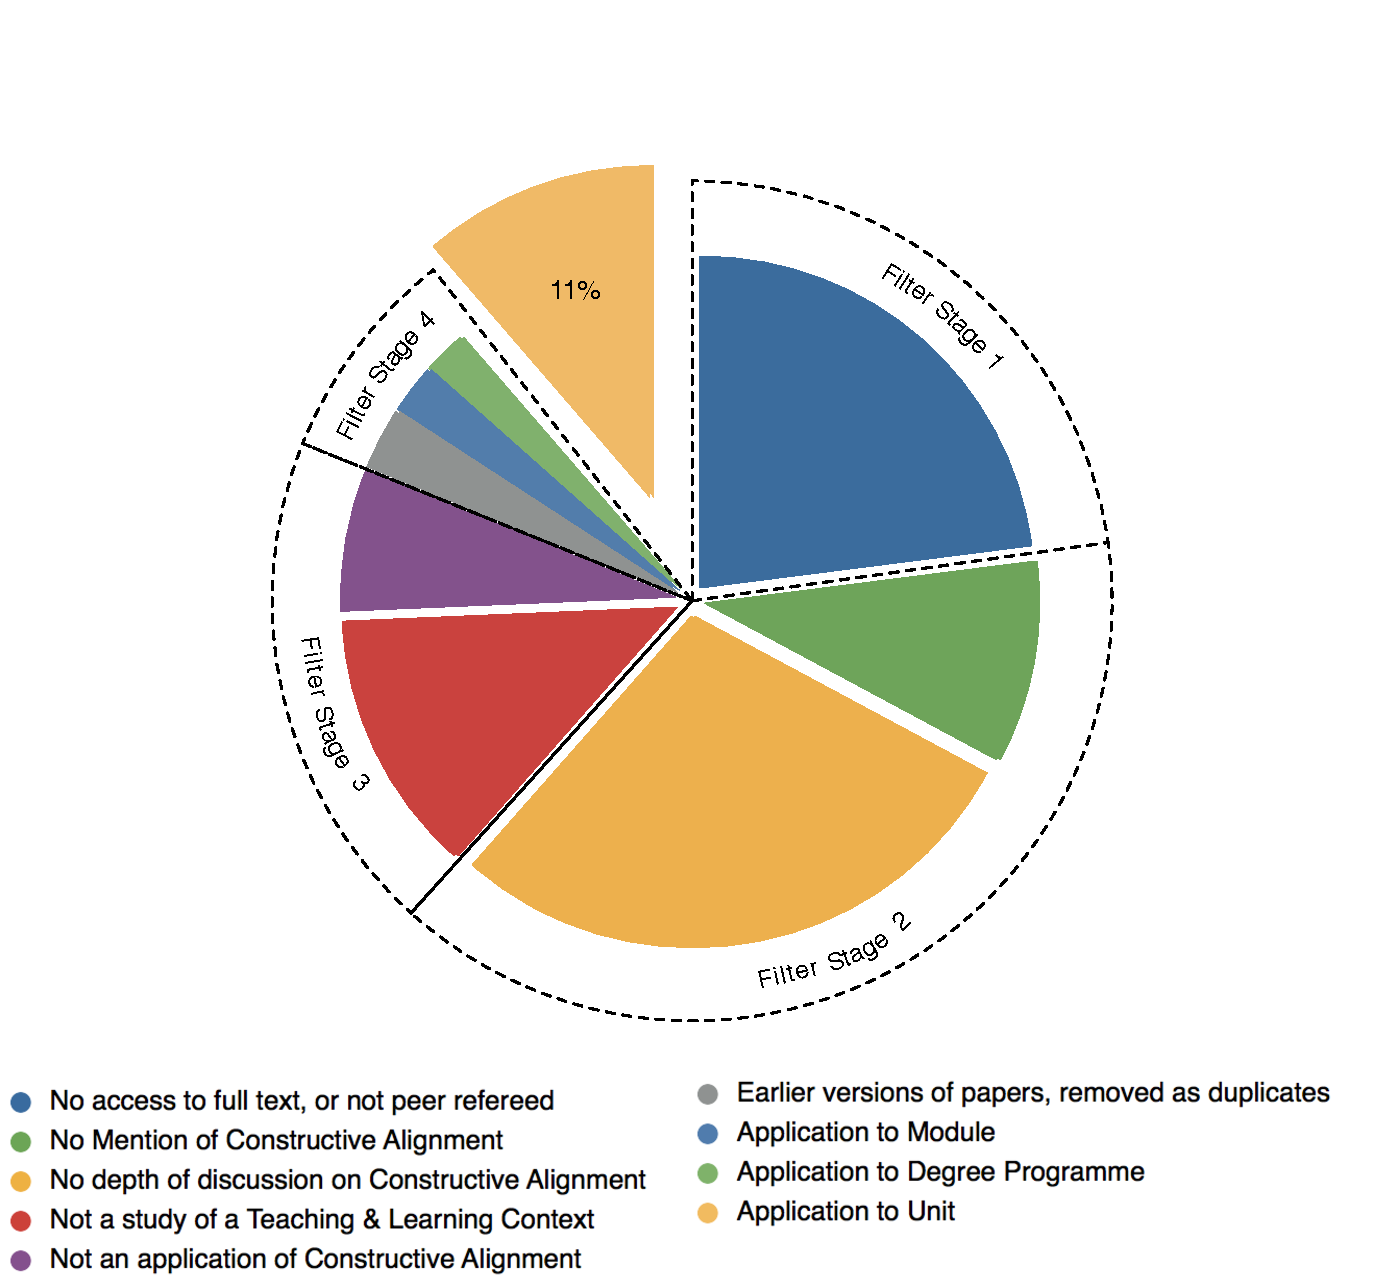
\includegraphics[width=\textwidth]{FilterResults}
	\caption{Pie chart showing the proportion of initial 335 papers in each status based on the stage excluded by the filters}
	\label{fig:filter_results}
\end{figure}

\subsubsection{Overview of Papers Collected} % (fold)
\label{sub:overview_of_papers_collected}

\tref{tbl:degrees} and \fref{fig:degree_dist} show the number of papers by field of study. This list uses the Fields of Study defined by \citet{Trewin:2000}, and each of the units described was allocated to one of the associated fields. A total of sixteen (42\%) of the papers were associated with the fields of Information Technology or Management and Commerce, with each field being associated with the units from eight papers. No papers were associated with Creative Arts, Food, Hospitality, and Personal Services, or Mixed Field Programmes.

\begin{table}[p]
	\centering
	\caption{The number of papers, from the 38 papers included in the analysis, in each field of study}
	\label{tbl:degrees}
	\footnotesize
    \begin{tabular}{lc}
    \textbf{Field} & \textbf{Count} \\ \hline
    Information Technology & 8 \\
	Management and Commerce &	8 \\
	Society and Culture &	6 \\
	Health &	4 \\
	Agriculture, Environmental and Related Studies &	3 \\
	Education &	3 \\
	Engineering and Related Technologies &	3 \\
	Natural and Physical Sciences &	2 \\
	Architecture and Building &	1 \\
	Creative Arts &	0 \\
	Food, Hospitality and Personal Services &	0 \\
	Mixed Field Programmes &	0 \\
    \end{tabular}
\end{table}

\begin{figure}[p]
	\centering
	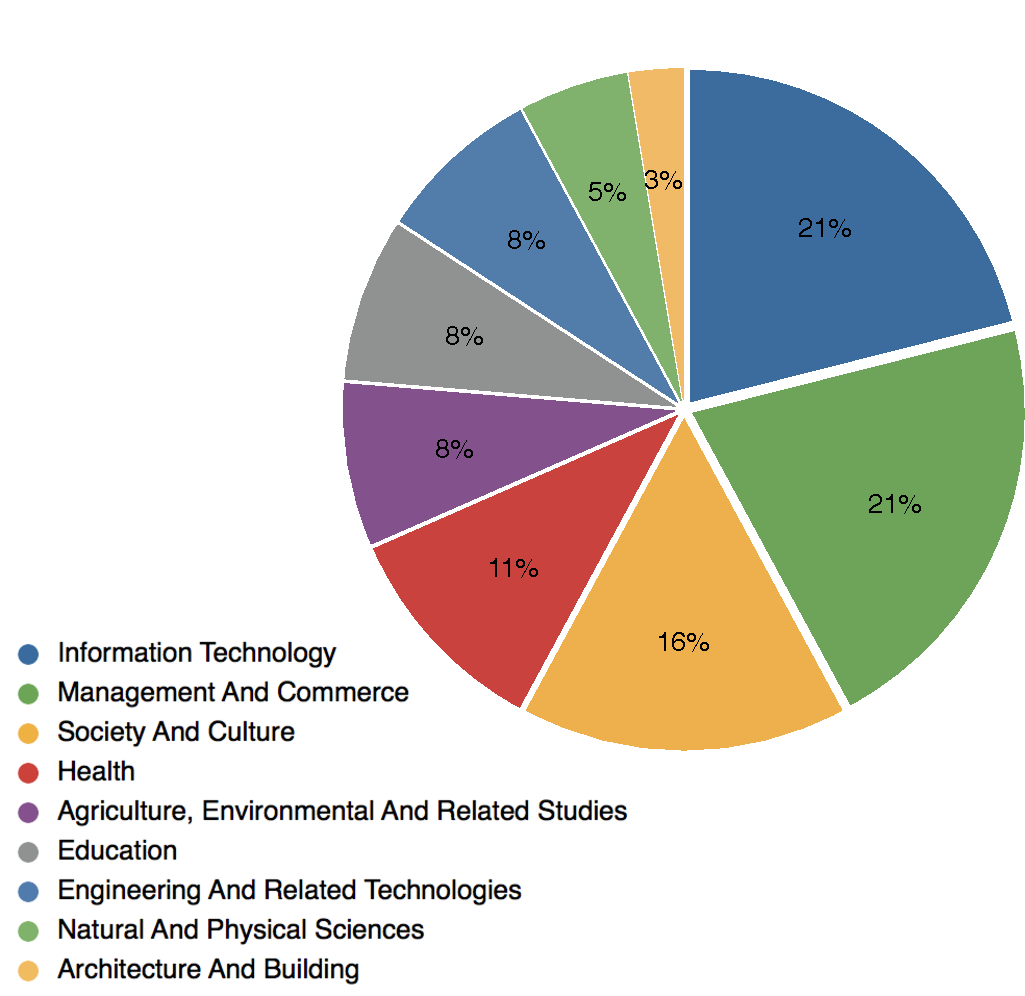
\includegraphics[width=\textwidth]{Degrees}
	\caption{Pie chart showing the distribution of papers by field}
	\label{fig:degree_dist}
\end{figure}

In terms of level of education, the analysed papers included units at both undergraduate and postgraduate levels. \tref{tbl:year_level} and \fref{fig:year_level} show the number of papers reporting units at the undergraduate and postgraduate levels. Where reported, the data collected includes the year level for undergraduate units. Two of the reported studies involved combined undergraduate and postgraduate units, and a further two units did not include any indication of the associated unit's level.

\begin{table}[p]
	\centering
	\caption{Numbers of papers reporting on units at undergraduate and postgraduate levels, and the indicated year level for undergraduate units.}
	\label{tbl:year_level}
	\footnotesize
    \begin{tabular}{lc}
    \textbf{Level and Year} & \textbf{Count} \\ \hline
		Undergraduate (Total)	 & 33 \\
		- First Year & 	7 \\
		- Second Year & 	5 \\
		- Third or Later Years	 & 12 \\
		- Year level not stated & 	9 \\
		Postgraduate & 	5 \\
		Level not stated & 2 \\
    \end{tabular}
\end{table}

\begin{figure}[htbp]
	\centering
	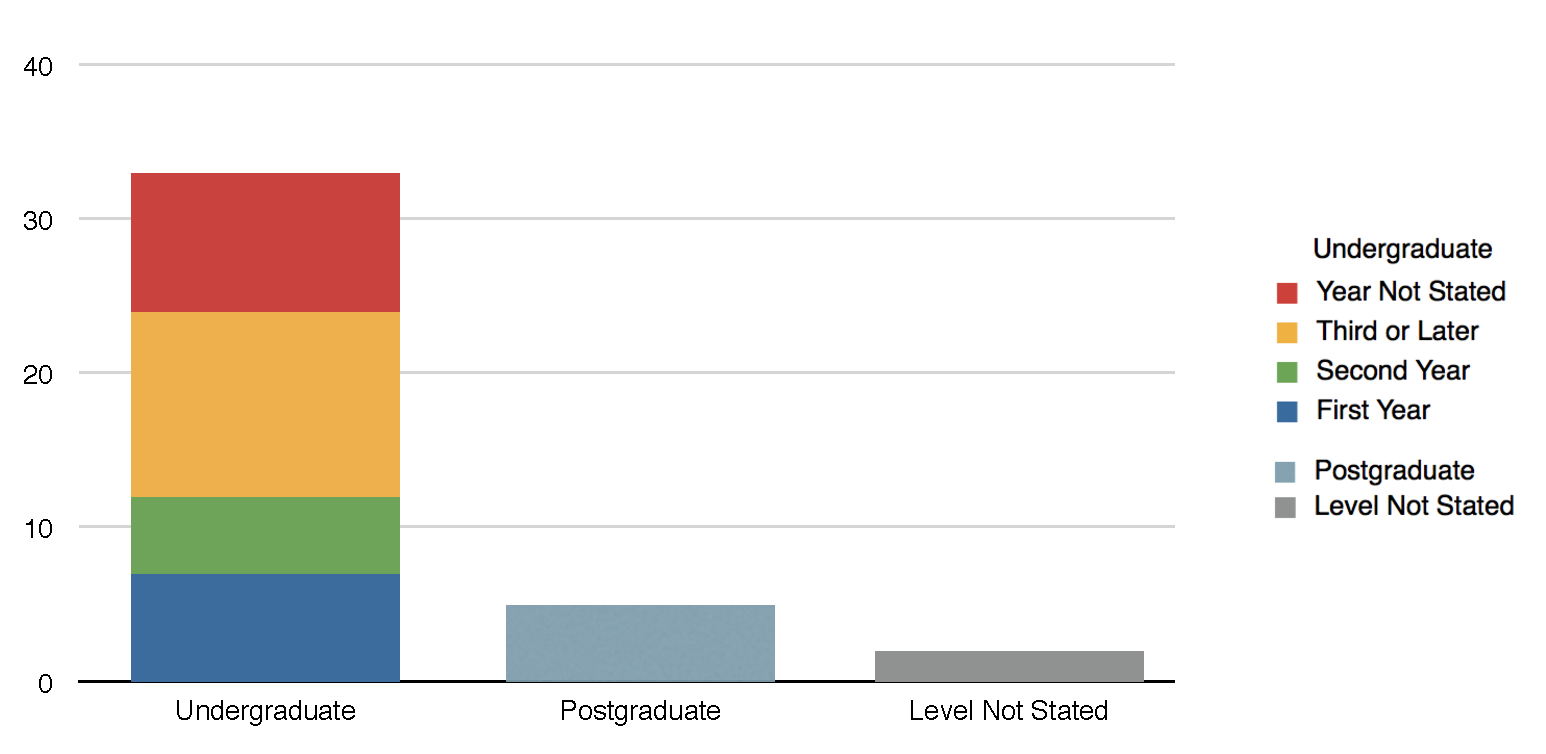
\includegraphics[width=0.8\textwidth]{LevelAndYear}
	\caption{Bar chart showing the level, and year, of the units reported.}
	\label{fig:year_level}
\end{figure}

Units in the analysed papers were primarily delivered face to face (82\%), with three being delivered online (8\%), and four units having a combination of online and face-to-face delivery. These results are included in \tref{tbl:delivery}.

\begin{table}[htbp]
	\centering
	\caption{Method of unit delivery}
	\label{tbl:delivery}
	\footnotesize
    \begin{tabular}{l|c}
    \textbf{Delivery} & \textbf{Count} \\ \hline
    Face to Face & 31 \\
    Face to Face \& Online & 4 \\
    Online & 3 \\
    \end{tabular}
\end{table}

\tref{tbl:location} shows the geographic location of unit delivery in the reported work. The location of the authors university was used in the cases where the geographic location was not explicitly mentioned in the paper's text. It is interesting to note that although papers were collected from international sources, 47\% of the papers analysed related to units delivered in Australiasia, with 39\% from Australian universities and 8\% from universities in New Zealand. 

\begin{table}[htbp]
	\centering
	\caption{Count of papers by geographic location where the unit was delivered.}
	\label{tbl:location}
	\footnotesize
    \begin{tabular}{lc}
    \textbf{Geographic Location} & \textbf{Count} \\ \hline
		Australia	 & 15 \\
		United Kingdom & 	7 \\
		Europe & 	5 \\
		New Zealand & 	3 \\
		Hong Kong & 	3 \\
		China & 	2 \\
		United States of America & 	1 \\
		Canada & 	1 \\
		South Africa & 	1 \\
    \end{tabular}
\end{table}

The increasing popularity of constructive alignment, at least in terms of papers reporting its application, can be seen by examining publication years. \fref{fig:year} provides a visual representation of this data, also shown in \tref{tbl:year}, and indicates an increasing number of papers published from 2005. It should be noted that the search was performed on the 18\textsuperscript{th} of July 2012, and therefore figures for 2012 only capture papers indexed by the source databases prior to this time. The data in \fref{fig:year} and \tref{tbl:year} also includes the counts of work that was excluded as duplicate studies, where the one study had been presented in a number of papers.

\begin{table}[p]
	\centering
	\caption{Year of publication for the papers analysed. Note that the count for 2012 is partial as the search was conducted on the 18\textsuperscript{th} of July 2012. Numbers in parenthesis indicate the number of papers removed in the filtering process as a duplicate of later papers included. }
	\label{tbl:year}
	\footnotesize
    \begin{tabular}{lc||lc}
    \textbf{Year} & \textbf{Count} & \textbf{Year} & \textbf{Count} \\ \hline
		1999	&	1	& 		2006	&	2		\\
		2000	&	1	& 		2007	&	3 (3)	\\
		2001	&	0	& 		2008	&	4 (1)	\\
		2002	&	1	& 		2009	&	6		\\
		2003	&	1	& 		2010	&	5 (2)	\\
		2004	&	1	& 		2011	&	4 (2)	\\
		2005	&	3	& 		\emph{2012}	&	\emph{6}	\\
    \end{tabular}
\end{table}

\begin{figure}[p]
	\centering
	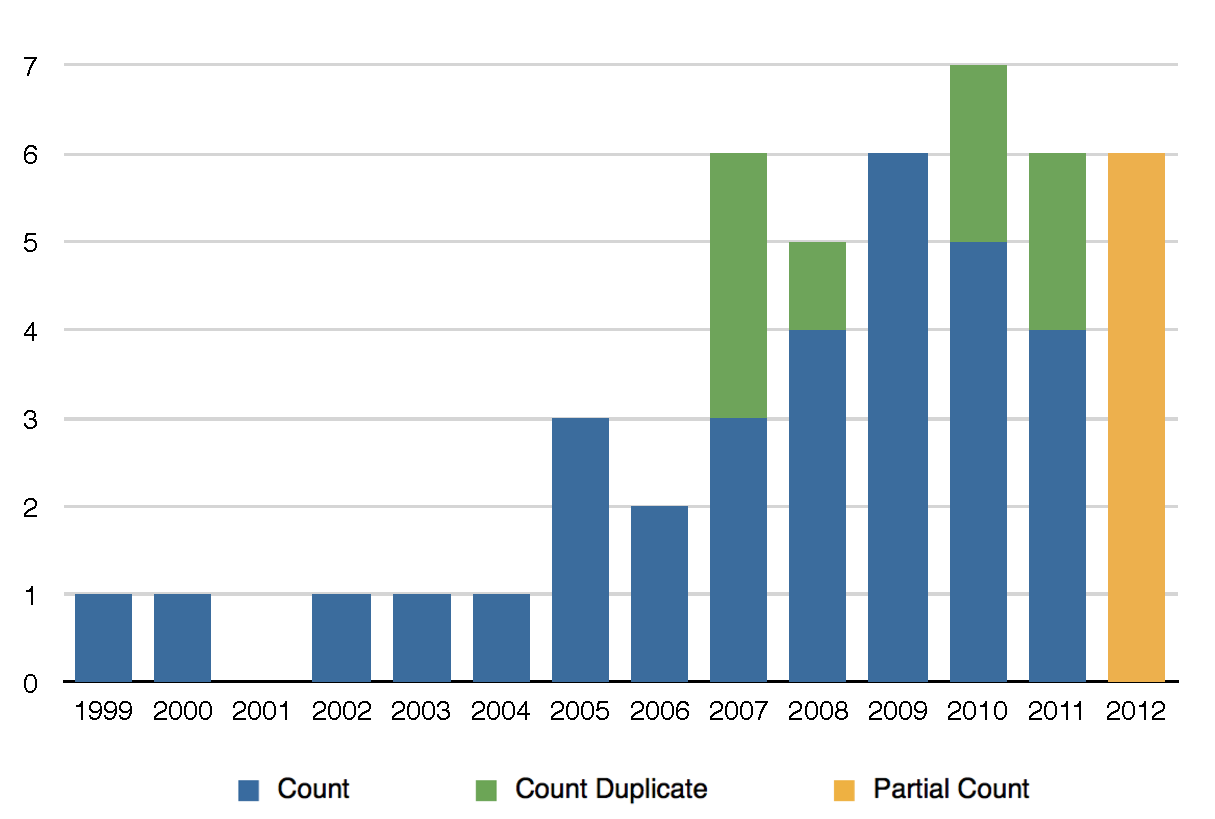
\includegraphics[width=\textwidth]{Year}
	\caption{Bar chart showing the number of papers published by year, including earlier versions of work included in the analysis, and the partial count of the papers published in 2012.}
	\label{fig:year}
\end{figure}


% subsection overview_of_papers_collected (end)
\subsubsection{Teaching and Learning Activities} % (fold)
\label{sub:teaching_and_learning_activities}

In the papers that included face-to-face delivery, the data collection examined the types of classes used. The results of this are included in \tref{tbl:class_types}, which lists the number, and percentage, of the papers that reported using lectures, various kinds of tutorials, and other teaching and learning activities. \tref{tbl:class_types} also records the number of papers in which there was no clear communication of the teaching and learning activities were used.

Lectures and tutorials remain the primary form of class used in the papers studied, with 74\% of the papers reporting either or both of these class types. Four papers included the use of \emph{Other} class types, the details of which appear in the following list. It is interesting to note that five papers (15\%) did not provide details on the teaching and learning activities used.

\begin{itemize}[noitemsep,nolistsep]
	\item \citet{Szili:2011} reported using a four day field camp to visit the scene of a serious environmental crisis, as part of a unit related to environmental management.
	\item \citet{donnisonre} included twenty hours of community service as part of a unit in the first year of an degree in Education.
	\item Eight weeks of clinical practice \citet{Tang:1999}, as part of a nursing degree.
	\item \citet{Shoufan:2010:CRP:1789934.1789937} included an excursion of a fabrication plant as part of an electronics and digital systems design unit. %, though this activity was not realted to the unit's outcomes. 
\end{itemize}

\begin{table}[htbp]
	\centering
	\caption{Class types used by units that included face to face delivery}
	\label{tbl:class_types}
	\footnotesize
    \begin{tabular}{l|c|c}
    \textbf{Class Type} & \textbf{Count} & \textbf{Percent} \\ \hline
    Lecture & 26 & 76\% \\
    Tutorial, Class, Workshop or Session & 25 & 74\% \\
    Other & 4 & 12\% \\
    Not reported & 5 & 15\% \\
    \end{tabular}
\end{table}

When collecting data on the class types used, additional information was sought as to how constructive learning theories had been incorporated into the teaching and learning activities. Three different strategies were identified: applying concepts through the use of \textbf{problem-based learning} or the examination of case studies, making the classes more \textbf{interactive}, and \textbf{group work} and discussions. 

Problem-based learning, projects, and case studies, all provide a means for educators to create a setting in which students can develop knowledge through application of associated principles. The constructivist nature of these activities has been reported by a range of authors. See for example, \citet{Hendry:1999,Savery:1995} and \citet{Schmidt:2009}. In the articles analysed in this research, examples of this approach include the use of Problem-based Learning by \citet{warren2005teaching} in teaching software design. Programming projects played an important part of the work reported by \citet{Brabrand:2008}, as these provided an opportunity for students to apply their understanding of concurrency in a practical sense.

\citet{Davey:2002} reported that in their unit on pharmacokinetics, lectures were changed to examine case studies that guided student decision making in relation to drug therapy and to explore scientific rationale. 

Interactive lectures and classes indicate a shift away from the objectivist ideas of knowledge transfer, and toward constructivist ideals. \citet{shepherd2005weaving} provides one example of this where lectures shifted to ``lectures as workshops'', with case studies being discussed and the lecturer solving problems from first principles.

\citet{Palincsar:1998} indicated that from a social constructivist perspective, higher-order thinking can be enhanced through the use of social interaction, such as can be achieved through classroom discussion. A number of papers indicated a shift to group work and classroom discussions as a means of engaging with these constructivist theories. One example of this shift is reported by \citet{Israel:2007}, who reported using tutorials as a means of guiding group research projects in their advanced undergraduate unit on psychology.

\begin{table}[tpb]
	\centering
	\caption{Method of incorporating constructive learning theories into the teaching and learning activities}
	\label{tbl:class_constructive}
	\footnotesize
    \begin{tabular}{l|c|c}
    \textbf{Method} & \textbf{Count} & \textbf{Percent} \\ \hline
    Applying Principles: Problem Based Learning, Projects or Case Studies & 18 & 53\% \\
    Moving beyond ``knowledge transfer'': Interactive Lectures and Classes & 11 & 32\% \\
    Social Constructivism: Group Work and Discussions & 9 & 26\% \\
    Not reported & 12 & 35\% \\
    \end{tabular}
\end{table}

\tref{tbl:class_constructive} shows the number of papers that reported the use different methods for incorporating constructive learning theories in the teaching and learning activities. Again, it is interesting to note that twelve papers (35\%) did not discuss the use of any method for addressing constructivism in their teaching and learning activities, which makes it difficult to understand how these papers adopted constructive learning theories, a key component of constructive alignment.

The remaining four online units used the following teaching and learning activities.

\begin{itemize}[noitemsep,nolistsep]
	\item \citet{hoddinott2000biggs} students were provided with reading, optional reading, and a range of online resources.
	\item \citet{raeburn2009blended} included work-based learning, and the use of online reflective journals.
	\item \citet{terrell2011using} provided online tutorials.
	\item \citet{brown2006looking} used online ``Thought Conferences'' where questions were designed to promote interaction through involving case studies and problem-based inquiry.
\end{itemize}

% subsection teaching_and_learning_activities (end)
\subsubsection{Approach to Student Assessment} % (fold)
\label{sub:review_assessment_approach}

Reported approach to student assessment included a range of activities, as shown in \tref{tbl:assessment_types}. Each of the different assessment approaches is detailed in the following list. % It is interesting to note that assignments and exams remain the most frequently used approach to assessment.

\begin{itemize}[noitemsep,nolistsep]
	\item \textbf{Examination}: Indicates the use of a final exam in the work.
	\item \textbf{Assignments}: Indicates the use of classwork assignments, projects, essays, and other work conducted by students individually during the teaching period.
	\item \textbf{Group Projects and Assignments}: Indicates the use of group marks in the student grades, and included group assignments, presentations and projects.
	\item \textbf{Reflective Journals}: Indicates the use of journals to reflect on the learning process.
	\item \textbf{Tests during delivery}: Indicates the use of tests commonly referred to as ``mid-term'' tests or quizzes.
	\item \textbf{Portfolios}: Indicates the use of a range of assessment approaches, discussed below, involving the collection of a number of pieces of work that are submitted as a group.
	\item \textbf{Participation}: Indicates that a part of the students grade was awarded for participation in teaching and learning activities.
\end{itemize}

\begin{table}[htbp]
	\centering
	\caption{Forms of assessment reported by the papers analysed}
	\label{tbl:assessment_types}
	\footnotesize
    \begin{tabular}{l|c|c}
     \textbf{Form of Assessment Used} & \textbf{Count} & \textbf{Percent} \\ \hline
No assessment specified & 	5 & 13\% \\
Assessment Specified	 & 33 & 	 \\
- Examination	 & 23	 & 70\% \\
- Assignments	 & 22	 & 67\% \\
- Group Projects and Assignments	 & 14	 & 42\% \\
- Reflective Journals & 	8	 & 24\% \\
- Tests during delivery & 	4	 & 12\% \\
- Portfolios & 	4	 & 12\% \\
- Participation &	2 & 	6\% \\
    \end{tabular}
\end{table}

Four papers indicated the use of portfolios in the student assessment but, unlike other forms of assessment, the exact nature of the portfolios differed between the various papers. It is interesting to note that the alignment between the portfolio and the unit's intended learning outcomes was not clearly presented in any of these four papers.

\begin{itemize}[noitemsep,nolistsep]
	\item \citet{Tang:1999} reported the use of a portfolio consisting of a learning diary, case study of a patient from clinical practice, and a piece of the students own choosing. This formed a part of the overall assessment along with an exam.
	\item \citet{raeburn2009blended} indicated the use of two portfolios, each of which included a resum\'{e}, a number of blog entries, and a written report of experience in work based learning. In this context a portfolio is simply a means of collecting together separate tasks.
	\item Portfolios reported by \citet{scott2009promoting} required students to complete twelve tasks over the course of the year, and combine these for submission as their portfolio. The assessment of the portfolio looked for ``positive contributions'', but little detail was provided as to how this assessment was performed.
	\item So called ``ePortfolios'' were used in conjuncture with other assignments in the work reported by \citet{donnisonre}. The ePortfolios included a multimedia digital story on the communities the students were involved with, and to document the student's community service experience.
\end{itemize}


% subsection assessment_approach (end)

\subsubsection{Aligning Curriculum and Assessment} % (fold)
\label{sub:aligning_curriculum}

All of the papers included some detail on curriculum alignment. In most cases the papers presented generic details of the importance of achieving alignment between teaching and learning activities and assessment tasks, with few actually providing any details on how this alignment was performed or specified. As indicated in \tref{tbl:alignment_details}, 61\% of the papers analysed provided little, or no, explicit details on how the alignment was achieved. In many of these papers the teaching and learning activities were discussed in some detail, but the specifics of how these were intended to develop the student's understanding of the intended learning outcomes was not discussed.

\begin{table}[p]
	\centering
	\caption{How alignment of teaching and learning activities, and assessment, was achieved as reported in the papers analysed.}
	\label{tbl:alignment_details}
	\footnotesize
    \begin{tabular}{l|c|c}
     \textbf{Aspect related to Alignment} & \textbf{Count} & \textbf{Percent} \\ \hline
	Alignment performed entirely by staff	 & 35	& 92\% \\
	&& \\
	Little, or no, explicit details about how alignment was performed	 & 23	& 61\% \\
	Explained alignment using matrix, graphic & 	9	& 24\% \\
	Explained using examples or textual explanations & 	6	& 16\% \\
    \end{tabular}
\end{table}

\begin{figure}[p]
	\centering
	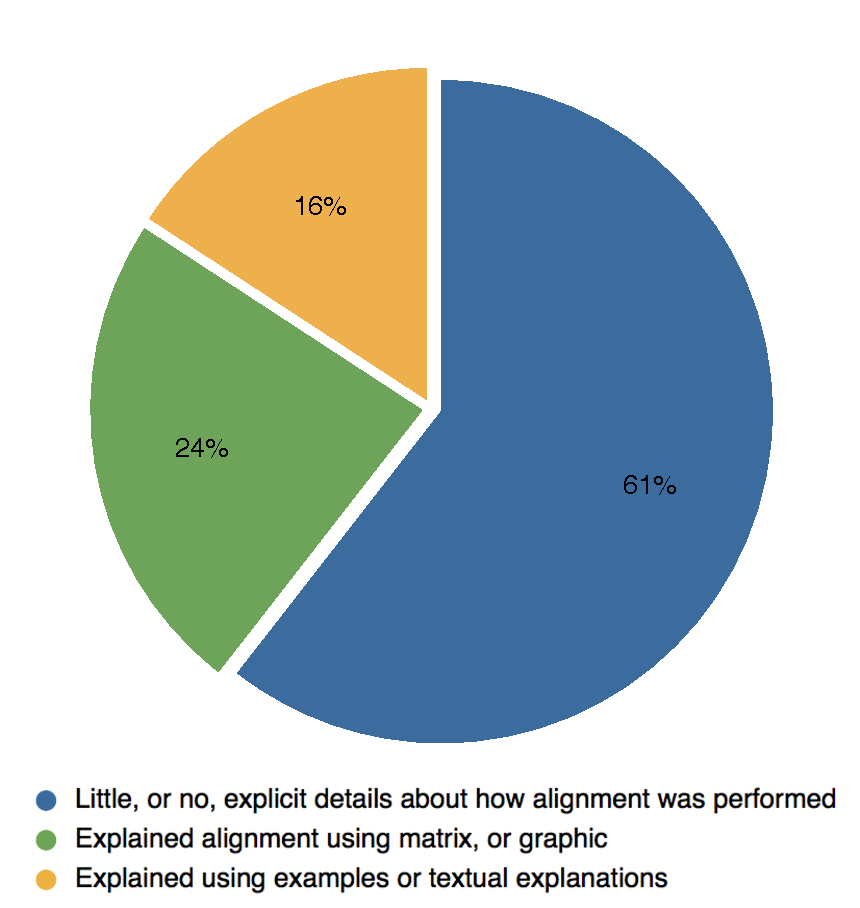
\includegraphics[width=0.5\textwidth]{AlignmentExplanation}
	\caption{Method used to explain the alignment of the curriculum}
	\label{fig:alignment_explain}
\end{figure}

Where an explanation of the alignment, the teaching and learning activities and assessment tasks were often presented in a matrix, or graphic, that showed the intended learning outcomes and the associated teaching and learning activities and assessment tasks. \tref{tbl:example_matrix} shows an example of how one of the intended learning outcomes was presented in \citet{terrell2011using}. Other papers included textual descriptions of how the alignment was performed. For example \citet{Brabrand:2008} provided an in-depth discussion of how they planned the alignment for their unit on concurrency. The numbers of papers that explained alignment using a matrix, other graphical means, or textually is shown in \tref{tbl:alignment_details} and graphically in \fref{fig:alignment_explain}.

\begin{table}[p]
	\centering
	\caption{Example of alignment matrix from \citet{terrell2011using}}
	\label{tbl:example_matrix}
	\footnotesize
    \begin{tabular}{p{4cm}|p{5cm}|p{3cm}}
     \textbf{Outcome} & \textbf{Activities} & \textbf{Assessment Criteria} \\ \hline
     \ldots & \ldots & \ldots \\
	\multirow{3}{4cm}{Using communication and team working skills to promote productive and cohesive relations among employees.} & 
	Read and comment on each other's blogs. & \multirow{3}{3cm}{Communication, Execution and Reflection} \\
	& Use Twitter to explore its use as a communication medium.
	&  \\
	& Share resources using social bookmarking tools\ldots & \\
	\ldots & \ldots & \ldots \\
    \end{tabular}
\end{table}

Thirty-five of the thirty-eight papers indicated that alignment was performed by staff. The remaining three papers included the use of portfolios where students were required to include evidence that aligned to the unit's intended learning outcomes. The relevant details from these three papers are described in the following list.

\begin{itemize}[noitemsep,nolistsep]
	\item \citet{hoddinott2000biggs} described a unit on Biology where students were required to align their portfolio submissions with the intended learning outcomes and assessment criteria. Unfortunately insufficient details were provided to enable deeper understanding of how this was subsequently assessed.
	\item Portfolios were also used in the unit described by \citet{scott2009promoting}, although no explicit details were provided about how alignment was achieved. 
	\item \citet{Tang:1999} provided a third example of portfolio assessment, but in this case the portfolio's objectives were not directly linked to unit intended learning outcomes.
\end{itemize}


% subsection aligning_curriculum (end)


% subsection results (end)

% section reported_applications_of_constructive_alignment (end)

\subsubsection{Reported Methods of Evaluation} % (fold)
\label{sub:method_for_evaluating_results}

The papers analysed indicated the use of one, or more, of a number of different data sources as a basis for their evaluation of the teaching and learning environment created. \tref{tbl:eval_source} lists the number of papers that included a single and multiple evaluation sources, and the number that did not include any evaluation.

\begin{table}[h]
	\centering
	\caption{Number of papers using a single, multiple, and no evaluation source.}
	\label{tbl:eval_source}
	\footnotesize
    \begin{tabular}{l|c}
     \textbf{Number of Sources} & \textbf{Count} \\ \hline
	Single Evaluation Source	 & 12 \\
	Multiple Evaluation Sources	 & 22 \\
	No Evaluation & 	4 \\
    \end{tabular}
\end{table}

Evaluations sources identified in the papers analysed are listed in \tref{tbl:eval_kind}, with each of the sources being described in the following list. 

\begin{itemize}[noitemsep,nolistsep]
	\item \textbf{Student Feedback} typically included feedback received as part of official unit evaluation questionnaires, but also included comments related to assessment tasks, and other informal sources of student feedback.
	\item \textbf{Results} indicated the use of unit grades, or results from individual assessment tasks.
	\item \textbf{Student Work} included document analysis of student assessment work, including assignments, examinations and portfolios.
	\item \textbf{Interviews and Focus Groups} additional feedback was received in response to focus groups or interviews in eight of the papers analysed.
	\item \textbf{Reflections on Teaching} staff reflections on teaching were included as a data source in four of the analysed papers.
	\item \textbf{Use of Online Tools} usage data from online learning management systems was used as a proxy for student engagement.
\end{itemize}


\begin{table}[b]
	\centering
	\caption{Evaluation sources used in the papers analysed}
	\label{tbl:eval_kind}
	\footnotesize
    \begin{tabular}{l|c}
     \textbf{Source Kind} & \textbf{Count} \\ \hline
		Student Feedback	 & 26 \\
		Results	 & 13 \\
		Student Work	 & 10 \\
		Interviews of Focus Groups & 	8 \\
		Reflection on Teaching & 	4 \\
		Use of Online Tools & 	3 \\
    \end{tabular}
\end{table}



% subsection method_for_evaluating_results (end)


\subsubsection{Reported Effects of Constructive Alignment} % (fold)
\label{sub:effects_of_constructive_alignment}

\tref{tbl:paper_results} lists the number of papers that indicated some positive results, or issues, in relation to the unit delivered. Of the thirty eight papers analysed, four did not include any evaluation of the delivery of the unit as noted in the previous section. Of the thirty four papers that included some results, 97\% indicated positive aspects and 21\% indicated issues.

\begin{table}[hbp]
	\centering
	\caption{Positive results and issues related to the teaching and learning environment created}
	\label{tbl:paper_results}
	\footnotesize
    \begin{tabular}{l|c|l}
     \textbf{Results} & \textbf{Count} & \textbf{Percent} \\ \hline
		No Evaluation & 	4 &	11\% of papers analysed \\
     	Results related to delivery & 34 & 89\% of papers analysed \\
		- Some Positive Results	 & 33 &	97\% of papers with results \\
		- Some Issues & 	7 &	21\% of papers with results  \\
    \end{tabular}
\end{table}

In relation to positive results, there were three common themes: positive learning outcomes, student satisfaction and student engagement. The number of papers reporting each of these is shown in \tref{tbl:pos_results}. Papers that reported other positive results are also included, and outlined in the following list.

\begin{itemize}[noitemsep,nolistsep]
	\item \citet{Hill:2009} reported benefits related to the ongoing refinement of the intended learning outcomes, and learning environment in general. The work also indicated that staff found the formative feedback was easier to deliver and stimulated wider discussion in class.
	\item \citet{Morton:2008} identified positive aspects related to improvements in written communication and understanding of the rigour required in laboratory work.
	\item Improvements in student confidence was reported by \citet{scott2009promoting}, along with their analysis of portfolios showing students had very deep and meaningful learning experiences.
	\item \citet{Schaefer:2009} reported that the use of real-world problems, as compared to textbook learning, had helped better prepare students for careers in mechanical engineering.
	\item \citet{Vanfretti:2011} indicated the use of free and open source software had helped to engage students in deep approaches to learning.
	\item \citet{Vogel:2007} indicated some positive effects for students using constructively aligned learning support over those who had chosen not to use these options. 
\end{itemize}

Positive learning outcomes were reported in the form of higher pass rates, higher percentage of students passing on the first attempt, or as demonstrations of high quality student learning outcomes. \citet{Szili:2011}, for example, indicated that student learning journals had exceeded staff expectations, with student work showing capacity to evaluate information, learning to reason and construct arguments, engagement with and learning from the wider world, and other positive learning outcomes. Other examples include the work of \citet{warren2005teaching}, where students who sat the exam demonstrated the ability to apply material covered to solve new problems.

High student satisfaction was also reported in a number of papers, and typically refer to some form of unit evaluation survey.  \citet{shepherd2005weaving}, for example, indicated that students regarded their learning experience in the associated unit as uniquely, or unusually, satisfying. Their work also indicated that students did not enjoy rote memorisation but often feel it is required or the only possible approach in some units. Similarly, \citet{scott2009promoting} reported very high satisfaction rates, with overall feedback being very positive. Students identified the interactive lecture approach and online resources as hugely beneficial.

Student engagement was also reported as a positive result in a number of papers. \citet{Davey:2002} reported a significant shift with students being more interested in their learning experiences and how the unit encouraged these. The work noted that students' comments shifted away from concerns of assessment requirements, to interest in what they were learning. Survey results indicated student interest in the subject matter, enjoyment of learning, and challenge and motivation to learn were significantly different after the reported initiative. Another good example of student engagement was reported by \citet{Szili:2011}, whose work showed students had a strong motivation for active participation in study and learning. Szili and Sobels cited their most important insight as the way that constructive alignment had worked seamlessly to deliver students who were motivated to pursue lifelong learning and engagement with their communities.

\begin{table}[htbp]
	\centering
	\caption{Papers that reported different kinds of positive results, and percentage compared to total number of papers reporting some positive results.}
	\label{tbl:pos_results}
	\footnotesize
    \begin{tabular}{l|c|c}
     \textbf{Positive Result Related To} & \textbf{Count} & \textbf{Percent} \\ \hline
	Learning outcomes (grades, or otherwise)	 & 19 &	58\% \\
	Student satisfaction	 & 17 &	52\% \\
	Student engagement & 	9 &	27\% \\
	Other positive aspects & 	6 &	18\% \\
    \end{tabular}
\end{table}

Problems arising from the application of constructive alignment were reported by only a few papers, with seven papers reporting issues related to the teaching and learning environment created. One common issue was additional staff and student workload as a result of the initiatives, as shown in \tref{tbl:neg_results}. Staff workload related to the development of new material, and the provision of feedback. Student workload issues were reported via the student satisfaction surveys. The remaining two issues, classified as other in the table, are detailed in the following list.

\begin{itemize}[noitemsep,nolistsep]
	\item \citet{Lin:2004} indicated that the less capable students may have found the problem-based learning approach used too complex and challenging.
	\item \citet{Tang:1999} reported students not enjoying the portfolio process, and not seeing it as contributing to their learning in the unit. This was attributed to either lack of clear instruction and support throughout the process, or to students prior expectations of assessment.
\end{itemize}

\begin{table}[htbp]
	\centering
	\caption{Papers that reported different kinds of issues, with percentage compared to total number of papers reporting at least one issue.}
	\label{tbl:neg_results}
	\footnotesize
    \begin{tabular}{l|c|c}
     \textbf{Negative Result, or Issues, Related To} & \textbf{Count} & \textbf{Percent} \\ \hline
	Staff Workload	& 2	& 29\% \\
	Student Workload	& 5	& 71\% \\
	Other	& 2	& 29\% \\
    \end{tabular}
\end{table}


% subsection effects_of_constructive_alignment (end)

\clearpage
\subsection{Discussion} % (fold)
\label{sub:discussion}


\subsubsection{Papers Identified} % (fold)
\label{ssub:geographic_location}

The use of a highly selective search criteria identified a wide range of papers, that were subsequently filtered to identify the papers analysed in this work. While every care was taken in filtering these papers, it is possible that a small number of papers were inappropriately excluded. To help mitigate this risk, the papers excluded at each stage were examined at least twice before filtering proceeded to the next stage. At the end of the process we have reasonable confidence in the papers included in this analysis.

It is concerning to note the number of papers that were excluded as a result of insufficient discussion on constructive alignment. Many of these papers included some details of constructive alignment in the introduction and background, and again in the conclusions, but provided no detailed discussion in the body of the work. For example, \citet{Penaluna:EducationTraining:2009} indicated opportunities for constructive alignment in the implications of their research on assessment strategies for entrepreneurship education, but provided no details on either constructivism or alignment in the remainder of the paper. 

One possible explanation for this in the wider field is the growing expectation that work in education should include the principles of constructive alignment. This message is, for example, clearly communicated in the work of \citet{Haigh:2013} on successfully writing for the Journal of Geography in Higher Education. Given the large number of papers in this category it would be interesting to examine them in more detail to see how they do relate to constructive alignment. 

The papers identified in this work provided a reasonable sample across a number of fields of study, but is predominantly related to undergraduate education. A greater balance between undergraduate and postgraduate had been expected, so it would be interesting to find out why constructive alignment has not been discussed more in relation to postgraduate education.

Examining the geographic location of the work resulted in a couple of interesting observations. Firstly the high number of papers from Australiasia, and the relatively small number from Northern America. The high number of papers from Australiasia may be a result of the choice of databases, with three of the databases containing work predominantly from Australia and New Zealand. However, the largest number of papers were located from databases with broad focus from international contributions, so this may indicate a greater focus on education research in this region, and a wide adoption of the principles of constructive alignment. The reverse could therefore also be posed in relation to the relatively small number of papers from Northern America. This could indicate that constructive alignment has not gained popularity in that region, or that relatively little research is published on the application of principles in Education. Both cases provide interesting questions for future research.

% subsubsection geographic_location (end)

\subsubsection{Effective Evaluation Sources} % (fold)
\label{ssub:effective_evaluation_sources}

A clear message from the analysed papers was the value of using multiple data sources in evaluating outcomes. Student satisfaction surveys and unit results appear to be readily available sources of information, and provide valuable evidence of learning outcomes and student perceptions. This can then be further enhanced by analysis of student work and staff reflections.

One topic not often discussed in the papers analysed is the ethical implications of using student work for purposes other than assessing the students learning. Issues related to the power imbalance of the student-teaching relationship, and issues associated with the perception of coercion need to be addressed. If student work is to be used then an appropriate ethical protocol needs to be developed, and students given the opportunity to give informed consent for their participation in the research.

% subsubsection effective_evaluation_sources (end)

\subsubsection{Opportunities for Misalignment} % (fold)
\label{ssub:opportinities_for_misalignment}

There appears to be significant opportunities for misalignment due to the lack of student engagement with the alignment process. Many of the papers analysed used a traditional assessment strategy involving the use of one, or more, assignments and a final exam. In this situation the teaching staff are entirely responsible for ensuring alignment between the unit's intended learning outcomes and the outcomes assessed in student submissions. 

\fref{fig:misalignment} tries to capture the situation where staff perform the alignment, for the purpose of illustrating areas for potential misalignment. Staff use intended learning outcomes in the design of assessment tasks for the students to perform. These tasks may aim to elicit outcomes that require high level cognitive activities such as explaining or reflecting on the application of some principles. Staff intentions must then be communicated to students via the assessment tasks, a complex activity that can be unintentionally undermined in a variety of ways. Even if the intentions can be captured perfectly, student interpretations of these expectations are likely to weaken any requirements. As indicated in \sref{sub:approaches_to_learning}, a number of students will aim to perform assessment tasks with as little effort as possible. These students will employ surface level approaches to learning where possible, and will not engage high level cognitive activities if possible. 

\begin{figure}[p]
	\centering
	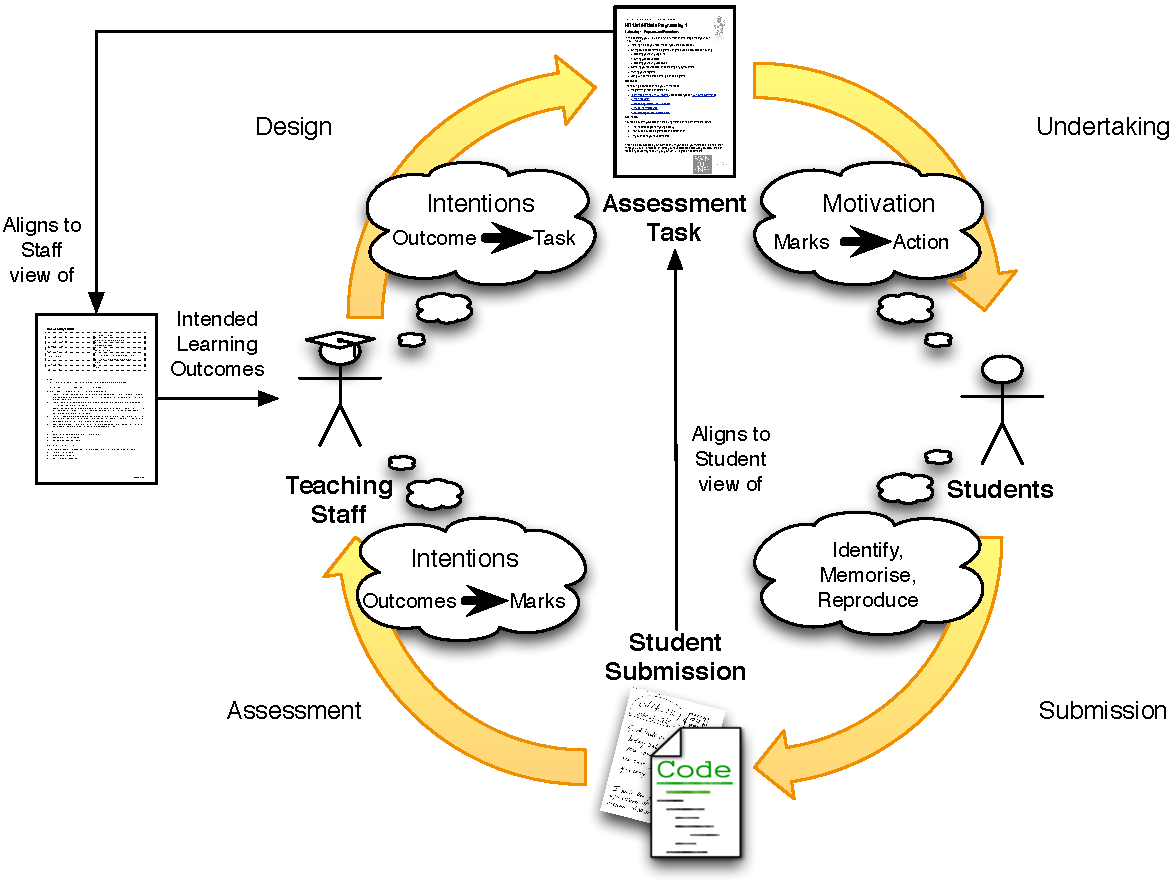
\includegraphics[width=\textwidth]{Misalignment}
	\caption{When using a traditional assignment and exam assessment strategy, particular attention is needed to ensure Staff intentions carry through to student actions.}
	\label{fig:misalignment}
\end{figure}

In addition to misalignment in the design of the assessment tasks there is also opportunities for misalignment on the assessment side of the process. Assessment tasks require assessment criteria that indicate how marks are awarded for the various aspects of the task. Where this is carried out quantitatively there is significant potential for misalignment, with the contents of knowledge needing to be broken down into identifiable units. As indicated by \citet{Biggs:1996c} this results in situations where assessment encourages piecemeal identification of details, and provides no encouragement for combining these details into a coherent whole.

Given the widespread and dominant use of assignments and exams and the potential for misalignment, it is particularly concerning how few papers provided any in-depth discussion on how the alignment was performed. Where details of the alignment were provided, the papers indicated how staff aligned topics in the intended learning outcomes with the tasks in the assignments and questions in the exams. However, few papers provided any reflections on the approaches that students had engaged, and how well these aligned with staff intentions. It should be mentioned that two of the papers analysed did provide good details on this aspect. \citet{Brabrand:2008} provided a very detailed discussion of how tasks had been aligned to outcomes, and yet still indicated that their work was not an ideal example of alignment in recognition of these challenges. \citet{Hill:2009} provided significant details on the challenges, and iterative improvements, with aligning student activity to outcomes and staff intentions with the delivery of their unit over a six years period. 

These challenges indicate that any genuine attempt to implement the principles of constructive alignment will need to be performed over a number of iterations. Each iteration should aim to improve alignment based on evidence gathered, and reflected upon, as part of unit delivery.

% subsubsection opportinities_for_misalignment (end)
 
\clearpage
\subsubsection{Business as Usual} % (fold)
\label{ssub:business_as_usual}

In proposing Constructive Alignment, \citet{Biggs:1996c} describes a teaching and learning environment which is student-centred. Biggs argued for the use of a range of teaching and learning activities, and encouraged active student engagement. With assessment, Biggs argued against examinations, short answer or multiple-choice questions. He indicated that these approaches to assessment are likely to give credit to lower level performances than intended, and thereby encourage students to adopt lower cognitive levels than desired. \citet{Biggs:1996c} strongly implied the use of portfolios, which was further elaborated upon in \citet{Biggs:1997}. Portfolio assessment in this context had referred to a body of work demonstrating how the student had met the intended learning outcomes, with a justification for how the selected pieces related to the unit objectives. The principles of Constructive Alignment had been discovered by Biggs as a result of the environment created through this clear focus on the intended learning outcomes, and the ``web of consistency'' that had resulted.

The clarity and vision provided by \citet{Biggs:1996c} does not appear to have resulted in many changes in the reported work. In many ways the papers analysed indicated a mostly ``business as usual'' approach. Constructive Alignment involved staff thinking about how their lectures, and the tasks they asked students to perform, related to the unit's intended learning outcomes. Some of the ideas of constructivism have made their way into teaching as either group work, and its associated group assessment, or attempts to make lectures and other classes more interactive. Similarly, approaches to assessment have remained primarily unchanged from the standard assignments and final exam. The ideas of learning through mistakes, and centring activities on students appears to have received little attention. Portfolios, when used, did not strongly follow the principles of Constructive Alignment, or had little details on how they had been implemented. 

% subsubsection business_as_usual (end)

% subsection discussion (end)


\clearpage
\section{Constructive Alignment in Introductory Programming} % (fold)
\label{sec:constructive_alignment_in_introductory_programming}

This section examines the topic of introductory programming in computing education research. It starts with an outline of challenges associated with introductory programming in \sref{sub:challenges_in_introductory_programming}. Following this is a description of published research perspectives on teaching introductory programming in \sref{sub:research_perspectives_on_introductory_programming}. The section concludes with a summary of two existing approaches to applying constructive alignment to introductory programming in \sref{sub:applying_constructive_alignment_to_introductory_programming}.

\subsection{Challenges in Introductory Programming} % (fold)
\label{sub:challenges_in_introductory_programming}

Introductory programming is a central skill for all students studying computer science and software engineering, and is often also taken by students in other fields. Units on introductory programming typically occur in students first year of university, and are widely recognised as being one of the most challenging units for these students. \citet{McGettrick:2005} described the need to better understand programming process and programmer practice so as to  deliver more effective educational outcomes as one of the seven grand challenges of computing education in recognition of the challenges related to teaching introductory programming.

Introductory programming can itself be viewed from a variety of perspectives. \citet{Dijkstra:1989} (see \citet{Denning:1989} for associated commentary) proposed a mathematical view of introductory programming, based upon formal methods and imperative programming. \citet{Palumbo:1990} discussed introductory programming from a problem solving perspective, with a focus on problem solving skills. \citet{DuBoulay:1986} likened programming to learning to control a notional machine, one that represents an ideal computer in which the programming constructs being taught are realised. However, in practice introductory programming units tend to follow a textbook style approach \cite{Robins:2003}, an approach that tends to focus on language syntax and illustrative examples. 

The goals of introductory programming have changed little in the last forty years. \citet{Gries:1974} indicated that introductory programming units should aim to teach students to solve problems, to describe an algorithmic solution to the problem, and verify that the algorithm is correct. These same concepts are at the core of all introductory programming units. This position was echoed by \citet{Marion:1999}, who commented that the advent of object oriented programming did not fundamentally change the objectives of introductory programming. Marion included objectives related to software design, algorithm design and analysis, problem solving, and language syntax necessary for expressing these ideas in a modern programming environment. In their study on what was taught in introductory programming, \citet{Schulte:2006} reported that most teachers taught such ``classic'' topics to the same extent, regardless of the approach they were using to teach the topic overall.

\citet{McCracken:2001} reported on an investigation of programming skills of first year computer science students across four universities. The investigators reported that results of the work were disappointing, and indicated that many students did not know how to program at the end of their first unit in introductory programming. A total of 216 students completed a \emph{Charette}, a short assessment carried out in a fixed-time laboratory session. The results included an analysis of the programs the students had completed, and indicated that in many cases students were not even able to produce code that compiled. Later work by \citet{Lister:2004} found similar results when examining students ability to determine output from small code snippets, known as ``code tracing tasks,'' and when selecting the code necessary to finish an almost complete piece of code. Given these poor results, gaining better understanding of the difficulties students face is an important avenue of research in the computing education research field.

Studies on novice programmers reported in \citet{Soloway:1988} indicated that novices have issues with many aspects of programming including concepts such as variables, loops, conditions, arrays, pointers and recursion, as well as having shortcomings related to planning and testing program code. The review of a number of psychological studies on programming by \citet{Winslow:1996} concluded that novices lacked appropriate ``mental models'' of computing, and so were limited to a surface understanding. This meant that student lacked sufficient structure to enable relevant aspects to be called upon when needed, with student approaching problems via control structures and line-by-line rather than by grouping into logical units. It is interesting to note that the work of \citet{Lahtinen:2005}, a survey 559 students across six universities, found that students also overestimate their understanding. This is likely to be related to their limited ``mental model'' and surface understanding of the subject, with many students failing to gain a relational level of understanding of the associated concepts. 

In reporting on their overview of research related to the psychology of programming, \citet{Robins:2003} indicate that novices face various problems, including issues related to; program design, ability to address algorithmic complexity, and the ``fragility'' of their knowledge, with learning to program requiring students to develop viable models of the problem domain, notional machine, and program structure. They found that students must then also develop skills necessary to map aspects from the problem domain to a the program structure, in such a way that this structure can effectively control the notional machine and generate the required outputs. The work also identified students as either ``effective novices'', who were able to learning to program with a reasonable effect, and ``ineffective novices'' who needed to expended an inordinate amount of effect to learn the required material.

Differences between effective and ineffective programming novices was reported by \citet{Renumol:2010}. The work used verbal protocol analysis to examined the cognitive processes used by nineteen novices. It was found that both effective and ineffective novices had used the same set of cognitive processes. A total of forty two cognitive processes were identified, and the work concluded that the use of so many cognitive processes made programming difficult, and the programming process complex to learn and practice.

A common theme across the various papers on introductory programming is that students struggle more with how and when to use programming structures than with programming language syntax. For example, \citet{Winslow:1996} indicated that students typically found it easy to generate syntactically correct statements once they understood what was required. Similar results were reported by \citet{Lahtinen:2005}, who indicated that the biggest problem students faced was not language details, but applying such details to solve new problems and in the creation of larger programming structures. 

Approach to learning also appears to be recognised as a factor in students success in learning to program. The work of \citet{DeRaadt:2005} and \citet{Bruce:2003}, previously discussed in \sref{sub:approaches_to_learning}, indicated that approach to learning does effect results in introductory programming units, and that students need to engage in deep approaches to learning. This is further supported by the work of \citet{Jenkins:2002} on difficulties students face in learning to program, which indicated that students face a range of challenges including cognitive factors related to learning styles and motivation. Jenkins and colleagues noted that many students' approach to learning was inadequate for them to succeed in introductory programming units, with motivation being a contributing factor \cite{Jenkins:2001,Forte:2005}.

% subsection challenges_in_introductory_programming (end)
\clearpage
\subsection{Research Perspectives on Introductory Programming} % (fold)
\label{sub:research_perspectives_on_introductory_programming}

Given the challenges involved in teaching introductory programming, this is a very active area in the field of computing eduction research. In their survey of literature on introductory programming, \citet{Pears:2007} identified four main categories: curricula, pedagogy, language choice, and tool support. 

Work on curricula has examined how introductory programming fits into the wider university computing curriculum, including recommendations for computing curricula by major professional computing societies \cite{CC2001,CC2008,CSC2013}. Other work in this area has included tailoring introductory programming content to meet the needs of students not enrolled in computer science majors, such as that reported in \citet{Guzdial:2005} and \citet{Forte:2005}.

Computing education research related to pedagogy of introductory programming examines a range of aspects related to teaching and learning. The work of \citet{BenAri:2001,Denning:1989,Dijkstra:1989,Hoare:1969,Palumbo:1990} and \citet{Robins:2003}, discussed earlier in this chapter, all relate to pedagogy. Other work in this area includes the work of \citet{Soloway:1986} who discussed the use of plans and schemas in problem solving and program design, with additional details on the use of these in teaching programming being reported by \citet{Rist:2004}. \citet{Green:1996} and \citet{Green:2000} discussed issues of cognitive load associated with various programming language elements and environments. While \citet{Eckerdal:2005} described five different levels of understanding related to what it means to learning programming; from a surface level where programming is seen as a study of a programming language and the program text, to a deep level where programming is seen as involving problem solving skills that can be taken beyond the programming unit. 

Language and, by association, paradigm choice is also widely studied. There exists a wide variety of papers on which programming language can and should be use in teaching introductory programming, including the work from \citet{Koffman:1988,Mody:1991,Roberts:1993,Brilliant:1996,Boszormenyi:1998,Howell:2003,Kelleher:2005,Bishop:2006,Mannila:2006,Mannila:2006a,Pendergast:2006,Maloney:2010} and \citet{Anik:2011}. There are also a large number of papers on the debate as to which programming paradigm should be used early in the curriculum. See for example \citet{Pattis:1993,Cooper:2003,Bennedsen:2004,Howe:2004,Astrachan:2005,Lister:2006a,Reges:2006} and \citet{Ehlert:2009}. These aspects, and the associated work, are considered in more detail in \cref{cha:example_impl}.

Research on tool support for introductory programming examines the use of software tools specifically designed to support the needs of novice programmers, including work on automated assessment by \citet{AlaMutk:2007} and \citet{Douce:2005}, visualisation \cite{Naps:2002}, and programming environments \cite{Gross:2005,Kelleher:2005,Kolling:2003,Mason:2013}.

% subsection research_perspectives_on_introductory_programming (end)

\subsection{Applying Constructive Alignment to Introductory Programming} % (fold)
\label{sub:applying_constructive_alignment_to_introductory_programming}

Constructive alignment has also been seen as an avenue for improving outcomes in introductory programming. The work of \citet{Armarego:2009} concluded that traditional teaching approaches did not align well with the requirements of the computer science and software engineering disciplines, and may actually inhibit students, both current and potential, from engaging with associated topics. In agreement with this we suggest that an effective means of applying constructive alignment to the teaching of introductory programming is, therefore, imperative. 

\citet{Thota:2010} and \citet{Gaspar:2012} have each aimed to use the principles of constructive alignment to enhance the teaching of introductory programming. \citet{Thota:2010} described the development and delivering of an object oriented introductory programming unit that aligned with cognitive and affective learning outcomes. While the work of \citet{Gaspar:2012} discussed how the principles of constructive alignment represented a need to explicitly cover programming thought processes in teaching introductory programming, but did not discuss an overall application of these principles to the development of an associated unit of study. 

The work of \citet{Thota:2010} proposed a holistic and constructively aligned approach to introductory programming that aligned teaching and learning activities and assessment tasks with cognitive and affective learning outcomes. The described unit involved five intended learning outcomes related to object oriented programming, listed in \fref{fig:thota_ilos}. Each of the intended learning outcomes was mapped to programming concepts and techniques, and then to the assessment activities using a tabular matrix as discussed earlier in \sref{sec:reported_applications_of_constructive_alignment}.

\begin{figure}[htpb]
	\centering 
	\fbox{
	\parbox{0.9\textwidth}{
	\begin{guidelines}{ILO}
		\item Demonstrate knowledge and understanding of essential facts and concepts, relating to OOP.
		\item Deploy appropriate theory, practices and tools for problem definition, specification, design, implementation, maintenance and evaluation of programs.
		\item Use object-oriented design as a mechanism for problem solving as well as facilitating modularity and software reuse.
		\item Work productively as part of a pair/team.
		\item Demonstrate ability for organisation and internalisation of values.
	\end{guidelines}
	}}
	\caption{Intended learning outcomes from \citet{Thota:2010}.}
	\label{fig:thota_ilos}
\end{figure}

Constructive learning theories were embedded by \citet{Thota:2010} through the use of group work and pair programming. Teaching and learning activities included interactive lecture and laboratory classes, and the use of role plays and oral presentations. Adaptive quizzes, peer feedback, and lecturer feedback provided students with a range of useful resources to learn from. The use of class diagrams and an interactive debugger also helped students comprehend critical aspects of objects and classes.

Assessment in the unit reported by \citet{Thota:2010} was divided up into a number of tasks based upon the intended learning outcomes, and included the use of quizzes (5\%), an exam (10\%), programming assignments (30\%), group project (50\%), classwork, and a journal (5\%). With an additional stipulation that all intended learning outcomes had to be met to a satisfactory level, though no indication of how this was checked was provided. 

\citet{Thota:2010} reported higher mean scores for deep approach to learning than surface approaches, using \citet{Biggs:2001} two-factor study process questionnaire (R-SPQ-2F). A positive relationship between deep approach to learning and course grades, and a negative relationship between surface approaches and grades, was reported but found to be not statistically significant. Informational resources were considered more important by students as a source of their learning, than collaboration, which group work being cited as a source of conflict in the unit.

Overall the work of \citet{Gaspar:2012} and \citet{Thota:2010} are representative of the work on applying constructive alignment in general. \citet{Gaspar:2012} refers to the principles of constructive alignment \cite{Biggs:1996c} as a means of suggesting a range of changes, but did not discuss embedding the principles more deeply. While \citet{Thota:2010} provide a more genuine attempt at embedding these principles throughout their unit, the use of traditional assessment approaches could easily have resulted in unintended misalignment, which can be further eroded through significant use of group marks in students final grades. In these contexts it is hard to see how any given student's learning outcomes relate to a unit's intended leaning outcomes.

% subsection applying_constructive_alignment_to_introductory_programming (end)

% section constructive_alignment_in_introductory_programming (end)
\clearpage
\section{Summary} % (fold)
\label{sec:closing_comments}

\citet{Biggs:1996c} vision of constructive alignment provided a strong and compelling argument for focusing on \textbf{student-centred} approaches to learning and assessment. Biggs' example unit demonstrated clear alignment between the intended learning outcomes and assessment, with learning activities providing students with the means of addressing these outcomes in the preparation of their portfolios. In contrast, the reported applications of constructive alignment have remained primarily \textbf{teacher-centred}, with teaching staff defining teaching and learning activities that are then assessed using traditional weighted assignments and exams.

While existing approaches examined in the literature review presented in this chapter can be argued to be applications of ``Constructive Alignment'', they do not appear to have captured the dramatic shift in thinking reported by \citet{Biggs:1996c}. The student-centred approach of the portfolios, with alignment to intended learning outcomes at their core, does not appear to have gone beyond Biggs' original work. If the papers analysed in this review are representative of ``Constructive Alignment'', then the work reported by Biggs goes beyond the core principles to capture additional aspects that are beneficial to student learning. Rediscovering these principles and trying to recreate the ``web of consistency'' is a worthwhile pursuit, and a goal of this research.

% section closing_comments (end)

% chapter background (end)